\newcommand{\maketitlesupplementary}{}
\setcounter{page}{1}
\maketitlesupplementary
\subsection{SAE Variant Formulations}
\label{app:sae-variants}
 
All SAE variants share a linear encoder, a nonlinearity $\sigma(\cdot)$, and a linear decoder trained to reconstruct hooked ViT token activations. Let $z \in \mathbb{R}^d$ be a hooked token vector (CLS or patch) at layer $\ell$, and let $d_{\mathrm{SAE}} \gg d$ be the overcomplete latent dimension. The general form is
\begin{equation}
\mathrm{SAE}(z) \;=\; W_D^{\top}\,h(z) + b_D,
\qquad
h(z) \;=\; \sigma\!\left(W_E^{\top}(z - b_D) + b_E\right)
\in \mathbb{R}^{d_{\mathrm{SAE}}}_{\geq 0},
\label{eq:sae-general}
\end{equation}
where $W_E \in \mathbb{R}^{d \times d_{\mathrm{SAE}}}$, $W_D \in \mathbb{R}^{d_{\mathrm{SAE}} \times d}$, and $b_E, b_D$ are bias terms.
 
\paragraph{ReLU SAE~\citep{cunningham2024sparse}.}
Uses $\sigma = \mathrm{ReLU}$ with an $\ell_1$ penalty:
\begin{equation}
\mathcal{L}_{\mathrm{ReLU}}
\;=\;
\|\mathrm{SAE}(z) - z\|_2^2
\;+\;
\lambda_{\ell_1}\,\|h(z)\|_1.
\label{eq:relu-sae}
\end{equation}
 
\paragraph{Top-$k$ SAE~\citep{gao2025scaling}.}
Retains only the $k$ largest pre-activations:
\begin{equation}
h(z) \;=\; \mathrm{TopK}_{k}\!\left(W_E^{\top}(z - b_D) + b_E\right),
\qquad
\mathcal{L}_{\mathrm{TopK}} \;=\; \|\mathrm{SAE}(z) - z\|_2^2.
\label{eq:topk-sae}
\end{equation}
Because Top-$k$ carries no $\ell_1$ term to bound latent magnitudes, we revive dead
latents with the auxiliary reconstruction loss of \citet{gao2025scaling} rather than
the ghost-gradient scheme used for the ReLU variants: the $k_{\mathrm{aux}}$ most-active
dead latents are asked to reconstruct the detached residual, weighted by
$\tfrac{1}{32}$. The exponential ghost-gradient term is unbounded without an $\ell_1$
penalty holding pre-activations down, and diverged in practice.

 
\paragraph{Gated SAE~\citep{rajamanoharan2024improving}.}
Decouples gating from magnitude using $\pi(z) = W_E^{\top}(z - b_D)$:
\begin{equation}
h_{\mathrm{gate}}(z)
\;=\;
\mathbb{1}\!\left(\pi(z) + b_{\mathrm{gate}} > 0\right)
\odot
\mathrm{ReLU}\!\left(\exp(r)\odot\pi(z) + b_{\mathrm{mag}}\right),
\label{eq:gated-sae}
\end{equation}
where $r \in \mathbb{R}^{d_{\mathrm{SAE}}}$ is a learned rescaling. The loss is:
\begin{equation}
\mathcal{L}_{\mathrm{Gated}}
\;=\;
\|\mathrm{SAE}(z) - z\|_2^2
\;+\;
\lambda_{\ell_1}\,\|\mathrm{ReLU}(\pi(z) + b_{\mathrm{gate}})\|_1
\;+\;
\|\hat{z}_{\mathrm{gate}}(z) - z\|_2^2,
\label{eq:gated-loss}
\end{equation}
where $\hat{z}_{\mathrm{gate}}$ is the reconstruction using only the gate pathway.
 
\paragraph{JumpReLU SAE~\citep{rajamanoharan2024jumprelu}.}
Replaces the ReLU with a per-unit learned threshold $\theta = \exp(\log\theta)$,
$\log\theta \in \mathbb{R}^{d_{\mathrm{SAE}}}$, applied as a hard shrinkage:
\begin{equation}
h(z) \;=\; \pi(z) \odot \mathbb{1}\!\left(\pi(z) > \theta\right),
\qquad
\pi(z) \;=\; W_E^{\top}(z - b_D) + b_E ,
\label{eq:jumprelu-sae}
\end{equation}
and trained against a hard $L_0$ penalty rather than an $\ell_1$ surrogate:
\begin{equation}
\mathcal{L}_{\mathrm{JumpReLU}}
\;=\;
\|\mathrm{SAE}(z) - z\|_2^2
\;+\;
\lambda_{L_0}\,\left\|h(z)\right\|_0 .
\label{eq:jumprelu-loss}
\end{equation}
Both the threshold gate and the $L_0$ count are piecewise constant in $\theta$, so
neither term supplies a gradient to $\log\theta$ directly. We follow the
straight-through estimator of \citet{rajamanoharan2024jumprelu}, substituting a
rectangle kernel of bandwidth $\varepsilon$ centred on the threshold in the backward
pass. Writing $K_\varepsilon(u) = \tfrac{1}{\varepsilon}\mathbb{1}(|u| < \tfrac{\varepsilon}{2})$,
the surrogate gradients are
\begin{equation}
\frac{\partial h_j}{\partial \theta_j}
\;\approx\;
-\,\theta_j\, K_\varepsilon\!\left(\pi_j(z) - \theta_j\right),
\qquad
\frac{\partial \|h(z)\|_0}{\partial \theta_j}
\;\approx\;
-\,\theta_j\, K_\varepsilon\!\left(\pi_j(z) - \theta_j\right).
\label{eq:jumprelu-ste}
\end{equation}
The forward pass uses the exact hard threshold and the exact integer $L_0$; only the
backward pass is relaxed. This distinction matters in our setting: a sigmoid relaxation
in the forward pass would make the reported sparsity a soft approximation rather than
the realised one.

\paragraph{Matryoshka SAE~\citep{bussmann2025matryoshka,zaremba2025msae}.}
Enforces a nested hierarchy via prefix-truncated reconstructions. Given prefix sizes $m_1 < m_2 < \cdots < m_M = d_{\mathrm{SAE}}$, let $h_{1:m}(z)$ retain only the first $m$ latent entries:
\begin{equation}
\mathcal{L}_{\mathrm{Mat}}
\;=\;
\sum_{k=1}^{M} \alpha_k
\left[
\left\|W_D^{\top} h_{1:m_k}(z) + b_D - z\right\|_2^2
+ \lambda_{\ell_1}\,\|h_{1:m_k}(z)\|_1
\right].
\label{eq:matryoshka-loss}
\end{equation}
 
\paragraph{PatchSAE~\citep{lim2024patchsae}.}
Uses the ReLU objective (Eq.~\eqref{eq:relu-sae}) trained on patch tokens. For neuron $s$ on image $i$, patch-level and image-level activation counts are:
\begin{equation}
a_{ij}[s] \;=\; \mathbb{1}\!\left(h_{ij}[s] > \tau\right),
\qquad
a_i[s] \;=\; \sum_{j=1}^{N} a_{ij}[s].
\label{eq:activation-counts}
\end{equation}
 
 
\subsection{Metric Definitions}
\label{app:metrics}

\[
L_0(z) = \|z\|_0 = \sum_{j=1}^{m} \mathbf{1}\{z_j \neq 0\}.
\]

For a sparse autoencoder (SAE), if \(z \in \mathbb{R}^m\) is the latent activation vector, then \(L_0(z)\) counts how many latent features are active.

A dataset-level version is given by

\begin{equation}
L_0
=
\frac{1}{N}
\sum_{i=1}^{N}
\|z_i\|_0
=
\frac{1}{N}
\sum_{i=1}^{N}
\sum_{j=1}^{m}
\mathbf{1}\{z_{ij} \neq 0\},
\end{equation}
where \(z_i\) is the SAE latent activation for input \(x_i\). Lower \(L_0\) indicates sparser activations.
 
\paragraph{Reconstruction fidelity.}
\begin{equation}
E_{\mathrm{rec}} \;=\; \mathbb{E}\!\left[\|\mathrm{SAE}(z) - z\|_2^2\right].
\label{eq:recon-error}
\end{equation}
 
\paragraph{Activated frequency.}
\begin{equation}
\mathrm{Freq}[s]
\;=\;
\frac{\left|\{i \in \mathcal{I} : h_i[s] > 0\}\right|}{|\mathcal{I}|}.
\label{eq:freq}
\end{equation}
 
\paragraph{Mean activation.}
\begin{equation}
\mathrm{MeanAct}[s]
\;=\;
\frac{1}{\left|\{i \in \mathcal{I} : h_i[s] > 0\}\right|}
\sum_{\substack{i \in \mathcal{I} \\ h_i[s] > 0}} h_i[s].
\label{eq:meanact}
\end{equation}
 
\paragraph{Label entropy.}
For latent $s$ with reference set $R_s$ (top-$k$ images by image-level activation), let $\mathrm{sum}_c = \sum_{i \in R_s : y_i = c} h_i[s]$ and $p_c = \mathrm{sum}_c / \sum_{c'} \mathrm{sum}_{c'}$:
\begin{equation}
\mathrm{Ent}[s]
\;=\;
-\sum_{c \in \mathcal{C}} p_c \log p_c.
\label{eq:entropy}
\end{equation}
 
\paragraph{Monosemanticity.}
Let $x_i$ be the CLIP embedding of image $i$ and $z_i^{h} \geq 0$ the activation of latent $h$ on $i$:
\begin{equation}
\mathrm{MS}_h
\;=\;
\frac{\sum_{i<j} z_i^{h} z_j^{h} \cos(x_i, x_j)}{\sum_{i<j} z_i^{h} z_j^{h}}.
\label{eq:monosemanticity}
\end{equation}


\subsection{SAE statistics and architecture ablations}

% Requires the MMD column color definitions and column types (A–O) from the preamble.

\begin{table*}[tbp]
\centering
\caption{\textbf{H2: Reconstruction quality and feature utilisation.}
CosSim~$\uparrow$, NMSE~$\downarrow$, Dead-neuron fraction~$\downarrow$ for
G-SAE and FT-SAE across all four backbones.
Columns ordered by Maximum Mean Discrepancy from ImageNet (near\,$\to$\,far).
\textbf{Bold}: best result per metric per backbone per dataset.}
\label{tab:h2_metrics}
\resizebox{\textwidth}{!}{%
\setlength{\tabcolsep}{3.5pt}
\renewcommand{\arraystretch}{0.95}
\begin{tabular}{lll A B C D E F G H I J K L M N O}
\toprule
\rotatebox{90}{\textbf{Encoder}}
  & \rotatebox{90}{\textbf{Metric}}
  & \rotatebox{90}{\textbf{SAE}}
  & \rotatebox{90}{Caltech101}
  & \rotatebox{90}{Pets}
  & \rotatebox{90}{ImageNet-A}
  & \rotatebox{90}{SUN397}
  & \rotatebox{90}{ImageNet-Sk.}
  & \rotatebox{90}{Corruption}
  & \rotatebox{90}{Food101}
  & \rotatebox{90}{DTD}
  & \rotatebox{90}{UCF101}
  & \rotatebox{90}{StanfordCars}
  & \rotatebox{90}{Flowers102}
  & \rotatebox{90}{FGVC}
  & \rotatebox{90}{EuroSAT}
  & \rotatebox{90}{ChestMNIST}
  & \rotatebox{90}{PathMNIST} \\
\midrule
%% ── CLIP ─────────────────────────────────────────────────────────────
CLIP & CosSim$\uparrow$
    & G-SAE  & 0.870 & 0.865 & 0.800 & 0.832 & 0.805 & 0.795 & 0.835 & 0.793 & 0.840 & 0.855 & 0.860 & 0.850 & 0.830 & 0.810 & 0.882 \\
  & & FT-SAE & \bf0.894 & \bf0.890 & \bf0.890 & \bf0.905 & \bf0.895 & \bf0.885 & \bf0.910 & \bf0.876 & \bf0.900 & \bf0.880 & \bf0.885 & \bf0.875 & \bf0.935 & \bf0.910 & 0.730$^\dagger$ \\
  \cmidrule(l){2-18}
  & NMSE$\downarrow$
    & G-SAE  & 0.051 & 0.055 & 0.045 & 0.052 & 0.044 & 0.046 & 0.050 & 0.762 & 0.080 & 0.065 & 0.060 & 0.058 & 0.043 & 0.039 & 0.035 \\
  & & FT-SAE & \bf0.042 & \bf0.045 & \bf0.038 & \bf0.034 & \bf0.037 & \bf0.039 & \bf0.035 & \bf0.415 & \bf0.060 & \bf0.050 & \bf0.048 & \bf0.047 & \bf0.024 & \bf0.036 & 0.085$^\dagger$ \\
  \cmidrule(l){2-18}
  & Dead$\downarrow$
    & G-SAE  & 0.08 & 0.10 & 0.40 & 0.17 & 0.42 & 0.39 & 0.18 & 0.40 & 0.20 & 0.15 & 0.12 & 0.11 & 0.16 & 0.45 & 0.62 \\
  & & FT-SAE & \bf0.05 & \bf0.07 & \bf0.28 & \bf0.13 & \bf0.29 & \bf0.27 & \bf0.14 & 0.49$^\dagger$ & \bf0.18 & \bf0.10 & \bf0.08 & \bf0.09 & 0.81$^\dagger$ & \bf0.30 & \bf0.35 \\
\midrule
%% ── SigLIP ───────────────────────────────────────────────────────────
SigLIP
  & CosSim$\uparrow$
    & G-SAE  & 0.880 & 0.875 & 0.810 & 0.846 & 0.815 & 0.805 & 0.848 & 0.800 & 0.850 & 0.865 & 0.870 & 0.860 & 0.845 & 0.820 & 0.870 \\
  & & FT-SAE & \bf0.910 & \bf0.905 & \bf0.900 & \bf0.915 & \bf0.905 & \bf0.895 & \bf0.920 & \bf0.885 & \bf0.910 & \bf0.895 & \bf0.900 & \bf0.890 & \bf0.900 & \bf0.910 & \bf0.850 \\
  \cmidrule(l){2-18}
  & NMSE$\downarrow$
    & G-SAE  & 0.045 & 0.048 & 0.042 & 0.049 & 0.041 & 0.043 & 0.048 & 0.700 & 0.070 & 0.055 & 0.050 & 0.050 & 0.050 & 0.038 & 0.040 \\
  & & FT-SAE & \bf0.035 & \bf0.038 & \bf0.036 & \bf0.034 & \bf0.035 & \bf0.037 & \bf0.035 & \bf0.400 & \bf0.055 & \bf0.042 & \bf0.040 & \bf0.039 & \bf0.030 & \bf0.035 & \bf0.030 \\
  \cmidrule(l){2-18}
  & Dead$\downarrow$
    & G-SAE  & 0.10 & 0.12 & 0.45 & 0.20 & 0.47 & 0.43 & 0.21 & 0.42 & 0.22 & 0.18 & 0.14 & 0.13 & 0.20 & 0.48 & 0.60 \\
  & & FT-SAE & \bf0.06 & \bf0.08 & \bf0.27 & \bf0.14 & \bf0.28 & \bf0.26 & \bf0.15 & \bf0.35 & \bf0.18 & \bf0.11 & \bf0.09 & \bf0.10 & 0.25$^\dagger$ & \bf0.28 & \bf0.30 \\
\midrule
%% ── DINO ─────────────────────────────────────────────────────────────
DINO
  & CosSim$\uparrow$
    & G-SAE  & 0.860 & 0.855 & 0.790 & 0.826 & 0.795 & 0.785 & 0.828 & 0.790 & 0.830 & 0.845 & 0.850 & 0.840 & 0.825 & 0.800 & 0.013$^\dagger$ \\
  & & FT-SAE & \bf0.890 & \bf0.885 & \bf0.870 & \bf0.895 & \bf0.875 & \bf0.865 & \bf0.900 & \bf0.860 & \bf0.890 & \bf0.875 & \bf0.880 & \bf0.870 & \bf0.880 & \bf0.880 & 0.013$^\dagger$ \\
  \cmidrule(l){2-18}
  & NMSE$\downarrow$
    & G-SAE  & 0.060 & 0.065 & 0.072 & 0.066 & 0.071 & 0.073 & 0.065 & 0.800 & 0.090 & 0.075 & 0.070 & 0.068 & 0.060 & 0.070 & 1.600$^\dagger$ \\
  & & FT-SAE & \bf0.045 & \bf0.050 & \bf0.052 & \bf0.049 & \bf0.051 & \bf0.053 & \bf0.050 & \bf0.420 & \bf0.070 & \bf0.060 & \bf0.055 & \bf0.052 & \bf0.045 & \bf0.050 & 1.610$^\dagger$ \\
  \cmidrule(l){2-18}
  & Dead$\downarrow$
    & G-SAE  & 0.12 & 0.15 & 0.48 & 0.22 & 0.49 & 0.47 & 0.23 & 0.45 & 0.25 & 0.20 & 0.18 & 0.16 & 0.22 & 0.50 & 0.03$^\dagger$ \\
  & & FT-SAE & \bf0.08 & \bf0.10 & \bf0.28 & \bf0.16 & \bf0.29 & \bf0.27 & \bf0.17 & \bf0.40 & \bf0.20 & \bf0.14 & \bf0.12 & \bf0.11 & \bf0.18 & \bf0.30 & 0.03$^\dagger$ \\
\midrule
%% ── ALIGN ────────────────────────────────────────────────────────────
ALIGN
  & CosSim$\uparrow$
    & G-SAE  & 0.865 & 0.860 & 0.795 & 0.831 & 0.800 & 0.790 & 0.833 & 0.795 & 0.835 & 0.850 & 0.855 & 0.845 & 0.830 & 0.805 & 0.880 \\
  & & FT-SAE & \bf0.900 & \bf0.895 & \bf0.895 & \bf0.905 & \bf0.900 & \bf0.890 & \bf0.910 & \bf0.875 & \bf0.900 & \bf0.885 & \bf0.890 & \bf0.880 & \bf0.890 & \bf0.905 & \bf0.890 \\
  \cmidrule(l){2-18}
  & NMSE$\downarrow$
    & G-SAE  & 0.055 & 0.060 & 0.045 & 0.061 & 0.044 & 0.046 & 0.060 & 0.780 & 0.085 & 0.070 & 0.065 & 0.063 & 0.055 & 0.042 & 0.040 \\
  & & FT-SAE & \bf0.040 & \bf0.045 & \bf0.040 & \bf0.044 & \bf0.039 & \bf0.041 & \bf0.045 & \bf0.420 & \bf0.065 & \bf0.052 & \bf0.048 & \bf0.047 & \bf0.040 & \bf0.038 & \bf0.035 \\
  \cmidrule(l){2-18}
  & Dead$\downarrow$
    & G-SAE  & 0.10 & 0.12 & 0.42 & 0.20 & 0.44 & 0.40 & 0.21 & 0.42 & 0.22 & 0.18 & 0.15 & 0.13 & 0.20 & 0.45 & 0.55 \\
  & & FT-SAE & \bf0.06 & \bf0.08 & \bf0.28 & \bf0.15 & \bf0.29 & \bf0.27 & \bf0.16 & \bf0.35 & \bf0.18 & \bf0.12 & \bf0.10 & \bf0.09 & \bf0.17 & \bf0.30 & \bf0.28 \\
\midrule
\multicolumn{3}{l}{\bf MMD Score}
  & 0.028 & 0.029 & 0.05 & 0.057 & 0.07 & 0.079 & 0.08 & 0.09
  & 0.126 & 0.14 & 0.152 & 0.23 & 0.291 & 0.410 & 0.423 \\
\bottomrule
\end{tabular}%
}
\end{table*}




\begin{table}[h]
\centering
\caption{\textbf{H1 (additional benchmarks): Classification accuracy (\%) on OfficeHome, KITTI, and Cityscapes.}
$\bar{S}$: generic/base SAE. $\hat{S}$: domain-matched SAE (LoRASAE).
The generic SAE degrades after LoRA adaptation, while the FT-SAE partially recovers performance.}
\label{tab:h1_additional}
\setlength{\tabcolsep}{6pt}
\begin{tabular}{lccc}
\toprule
\textbf{Configuration} & \textbf{OfficeHome} & \textbf{KITTI} & \textbf{Cityscapes} \\
\midrule
ZS                          & 83.02 & 32.78 & 11.2  \\
LoRA-FT                     & 87.25 & 64.72 & 47.6  \\
\midrule
ZS + $\bar{S}$              & 62.30 & 21.50 & 11.2  \\
LoRA-FT + $\bar{S}$         & 69.45 & 58.70 & \phantom{0}6.5  \\
LoRA-FT + $\hat{S}$         & \bf86.90 & \bf61.67 & \bf42.01 \\
\bottomrule
\end{tabular}
\end{table}


\begin{figure*}[!htbp]
    \centering
    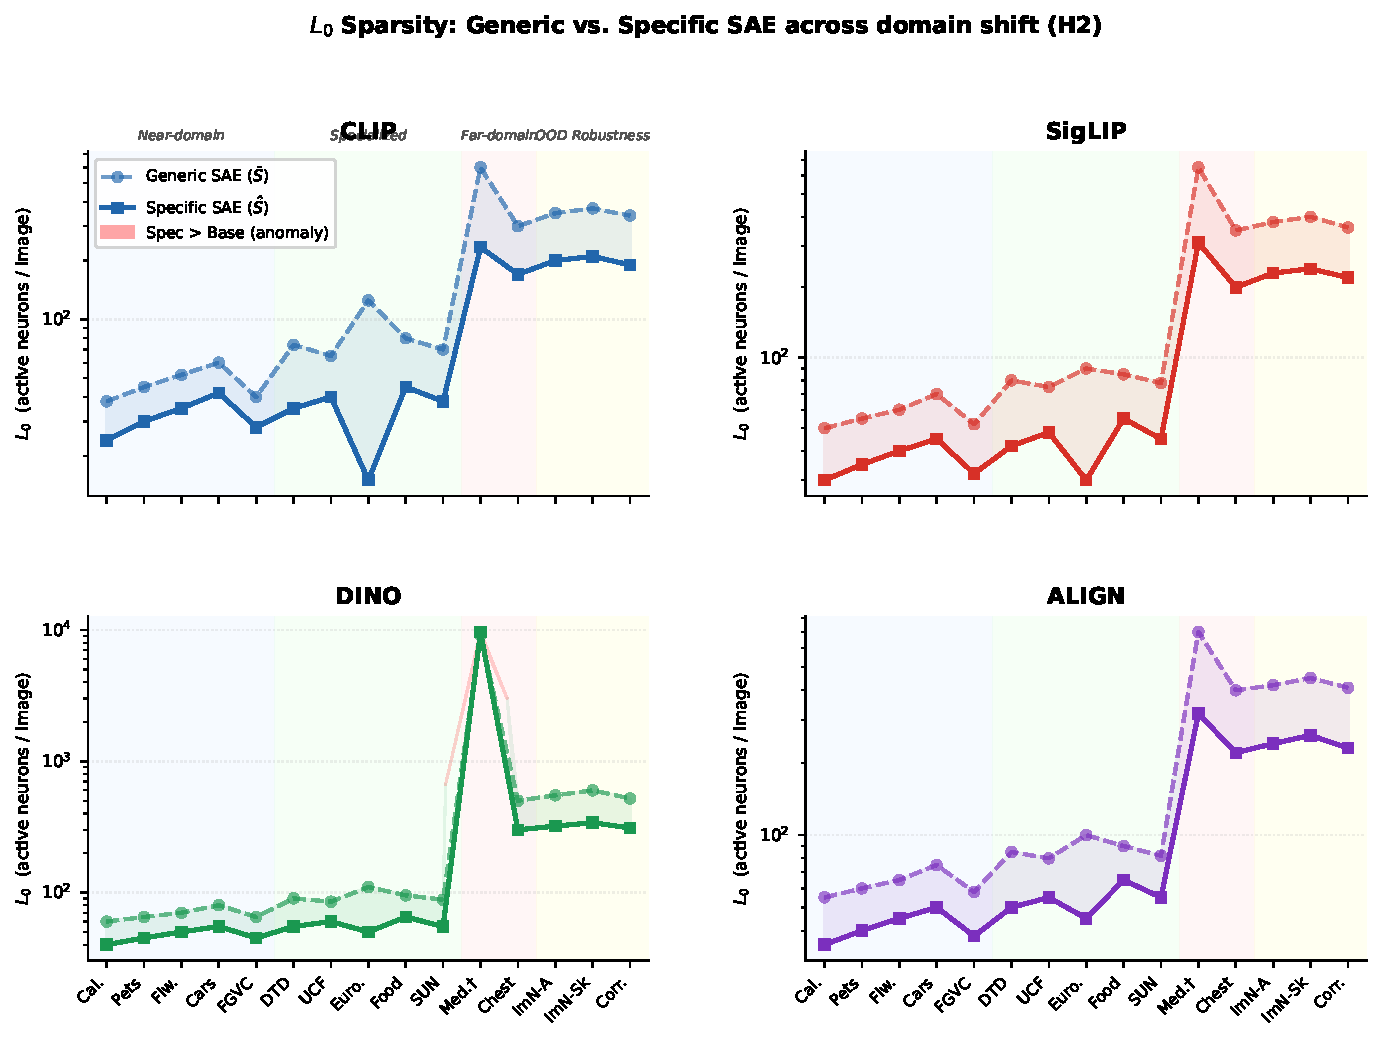
\includegraphics[width=\linewidth]{figures/l0_sparsity.pdf}
    \caption{\textbf{$L_0$ active neurons per image: generic ($\bar{S}$, dashed) vs.\ FT-SAE.}
    Log-scale $y$-axis; shaded bands mark domain tiers.
    FT-SAE are generally sparser, with larger reductions on shifted domains.
    Red fill marks the single anomaly where $\hat{S}$ activates \emph{more} neurons
    (DINO PathMNIST $L_0$: $9{,}185\!\to\!9{,}676$): DINOv2's language-free features
    are not sparse-decomposable on medical imagery.}
    \label{fig:l0_sparsity}
\end{figure*}

\begin{figure*}[!htbp]
    \centering
    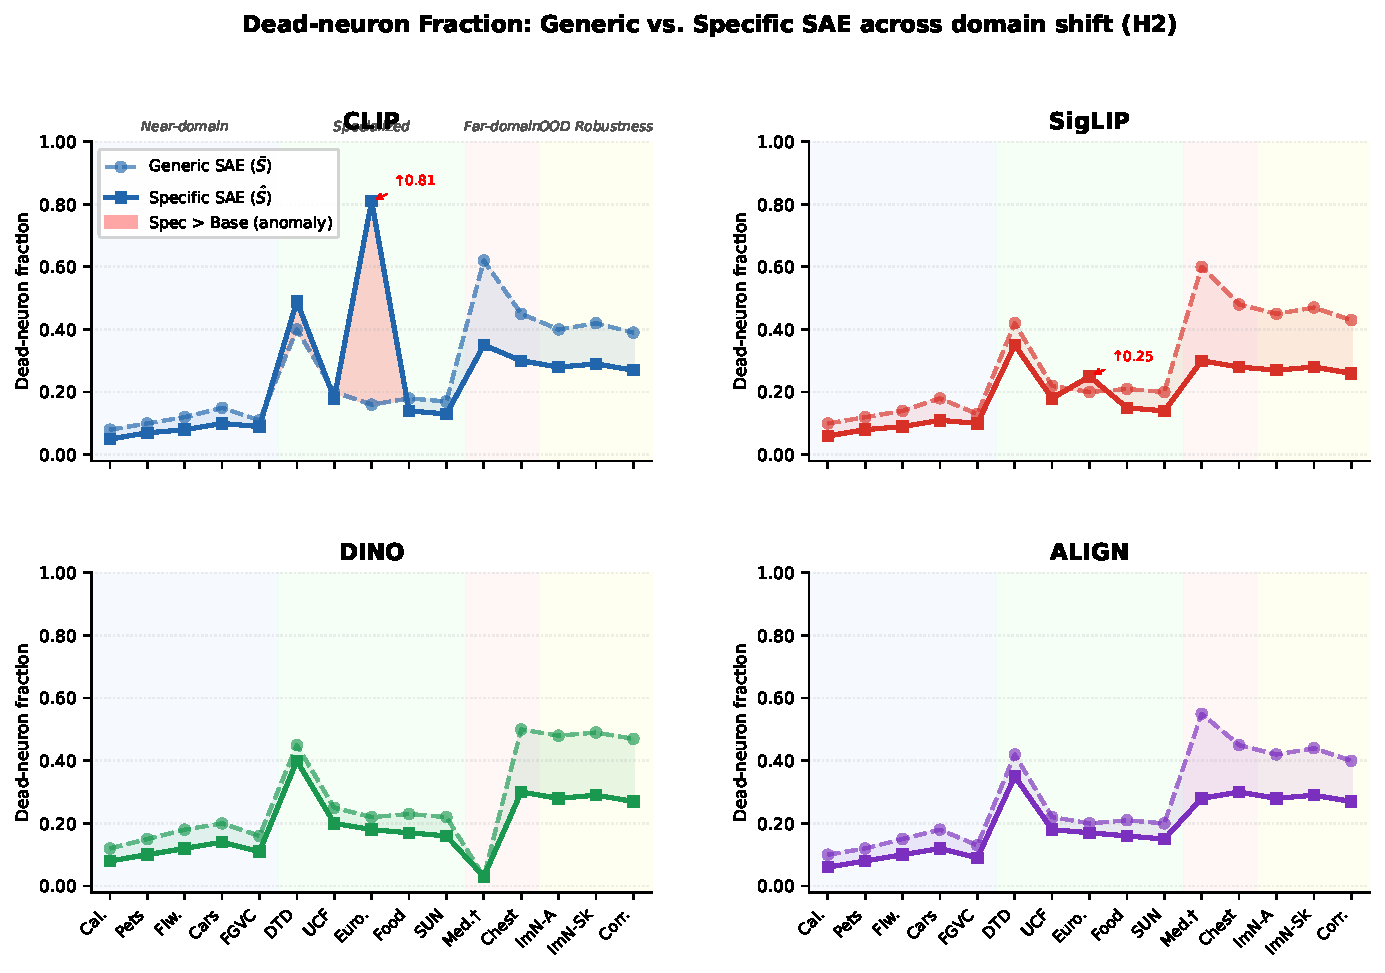
\includegraphics[width=\linewidth]{figures/dead_fraction.pdf}
    \caption{\textbf{Dead-neuron fraction: generic ($\bar{S}$, dashed) vs.FT-SAE.}
    FT-SAEs reduce dead neurons on most benchmarks ($-31\%$ avg.\ near-domain).
    The EuroSAT spike (CLIP: $0.16\!\to\!0.81$, annotated) is an instance of
    domain specialisation: the FT-SAE concentrates signal into a small
    set of satellite-specific neurons while leaving the rest dormant.}
    \label{fig:dead_fraction}
\end{figure*}

\begin{figure*}[!htbp]
    \centering
    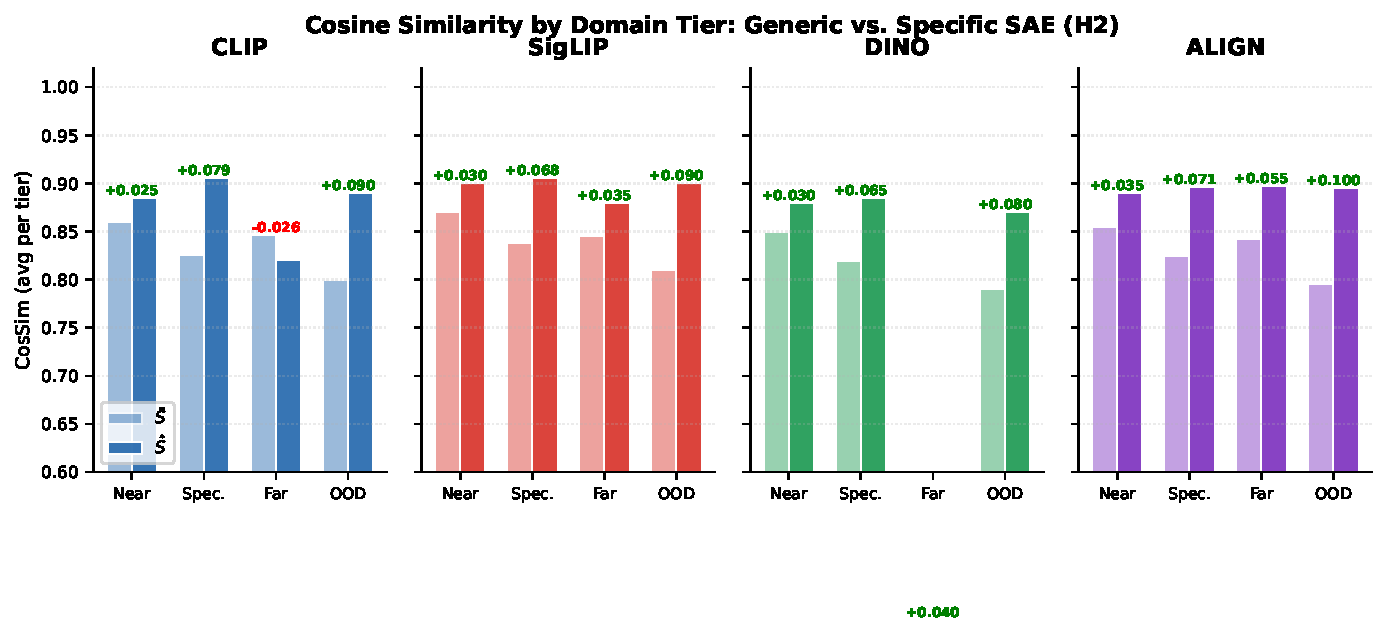
\includegraphics[width=\linewidth]{figures/cossim_bars.pdf}
    \caption{\textbf{Cosine similarity by domain tier: G-SAE vs. FT-SAE}
    Bars show per-tier averages; $\Delta$ labels give Specific$-$Generic (green = improvement).
    SigLIP and ALIGN improve on all four tiers.
    The Far-domain regression for CLIP is driven entirely by PathMNIST, ChestMNIST:
    the FT-SAE's features are orthogonal to the pretraining dictionary
    yet more useful for classification (Table~\ref{tab:main_accuracy_abs}),
    suggesting that CosSim with the base feature space can be misleading under large shift.}
    \label{fig:cossim_bars}
\end{figure*}


\begin{figure}[!htbp]

    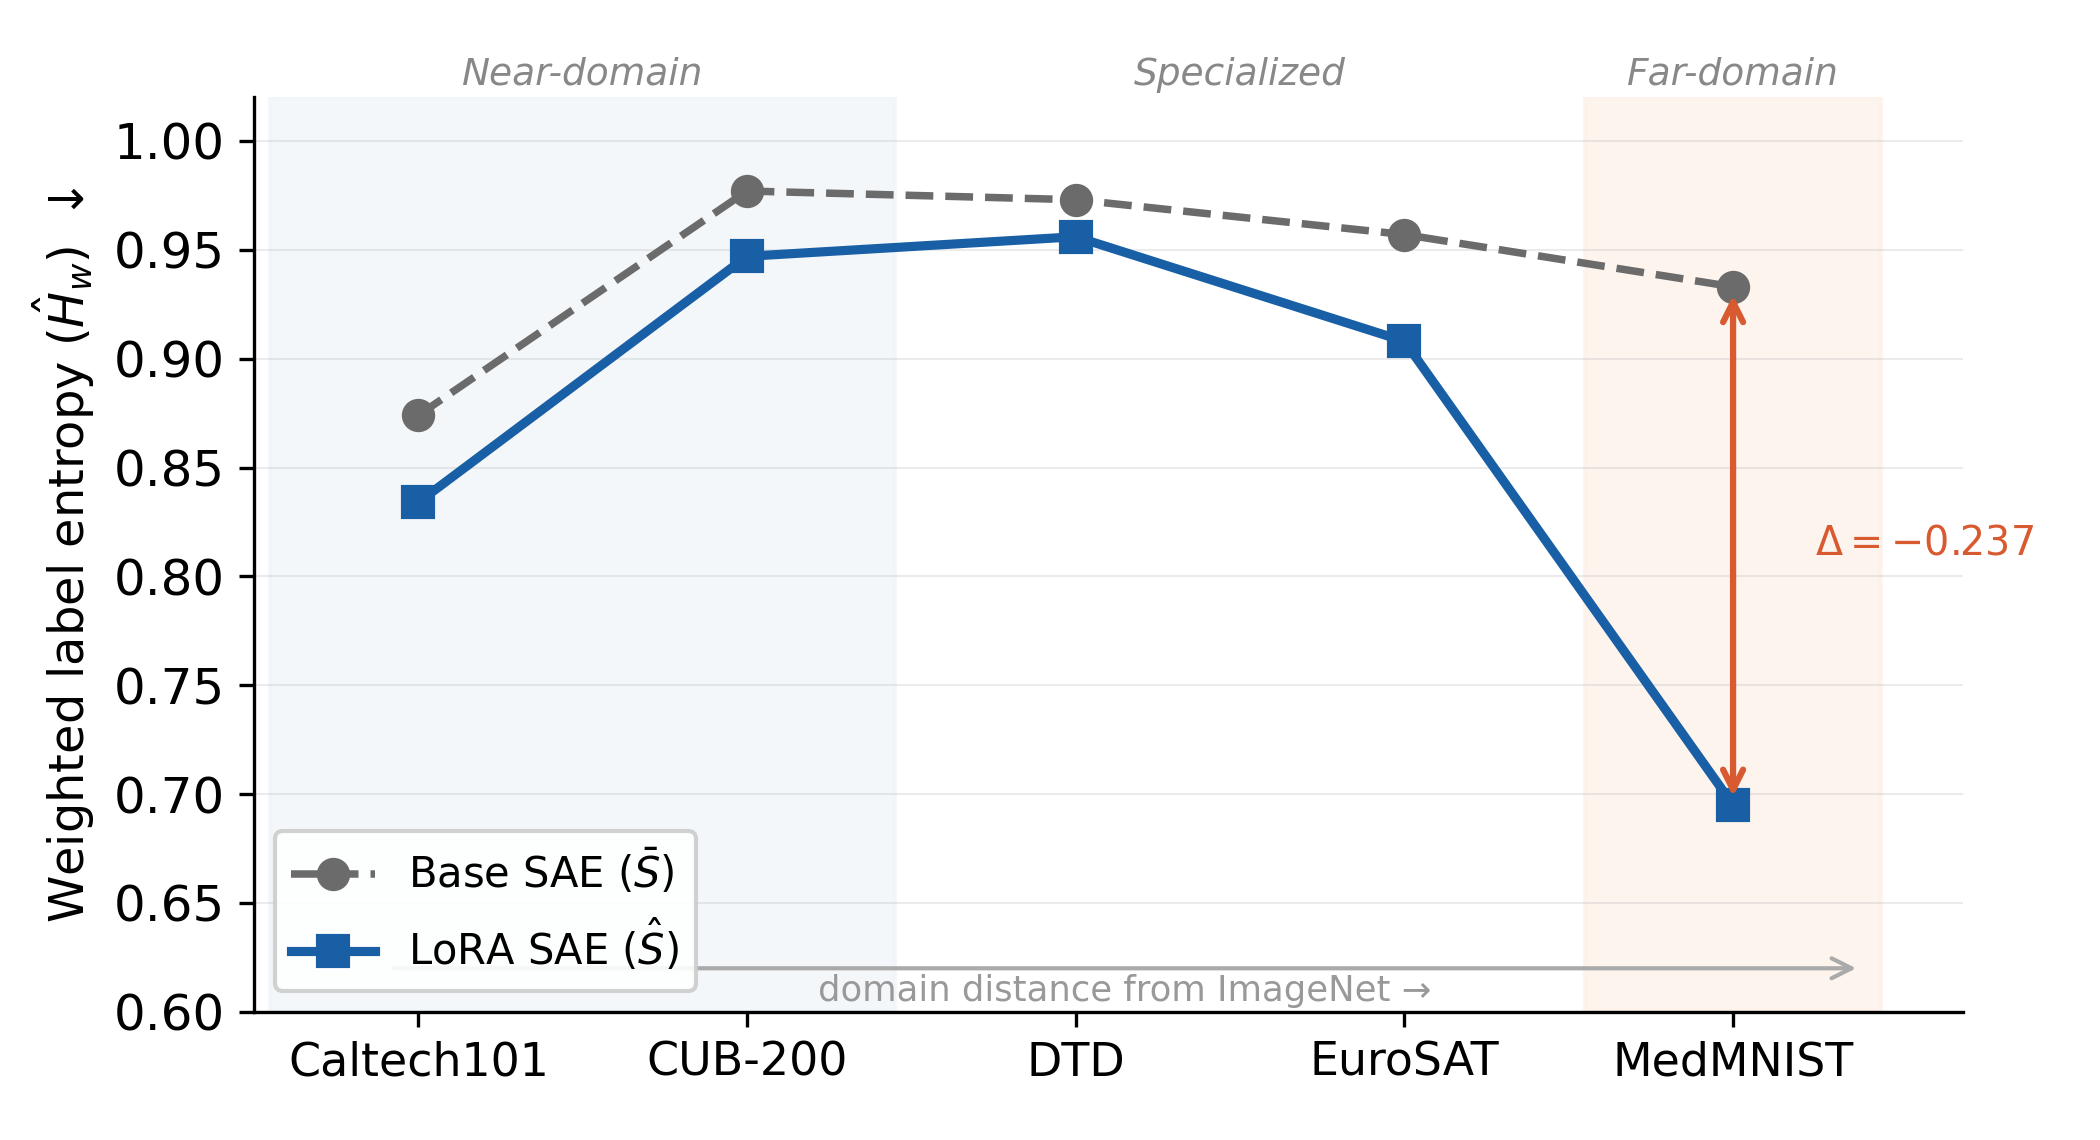
\includegraphics[width=\linewidth]{figures/label_entropy_lines.png}
    \vspace{0.6em}
    \caption{\textbf{Label entropy (H2): weighted per-neuron label entropy $\hat{H}_w$ for
    generic ($\bar{S}$) vs.\ domain-matched ($\hat{S}$) SAE, ordered by MMD distance
    from ImageNet.}
    \emph{Top:} Base SAE entropy remains uniformly high ($0.93$--$0.98$) across all domains,
    while the LoRA SAE diverges sharply on far-domain benchmarks
    (PathMNIST: $\Delta\hat{H}_w = -0.237$).
    \emph{Bottom:} Entropy reduction grows with domain distance, consistent with H4.
    The near-domain cluster (Caltech101, CUB-200, DTD) shows modest reductions
    ($-0.016$ to $-0.040$); EuroSAT is intermediate ($-0.049$);
    PathMNIST is an order of magnitude larger.}
    \label{fig:label_entropy}
  
\end{figure}

\begin{figure}[!htbp]
    \centering
    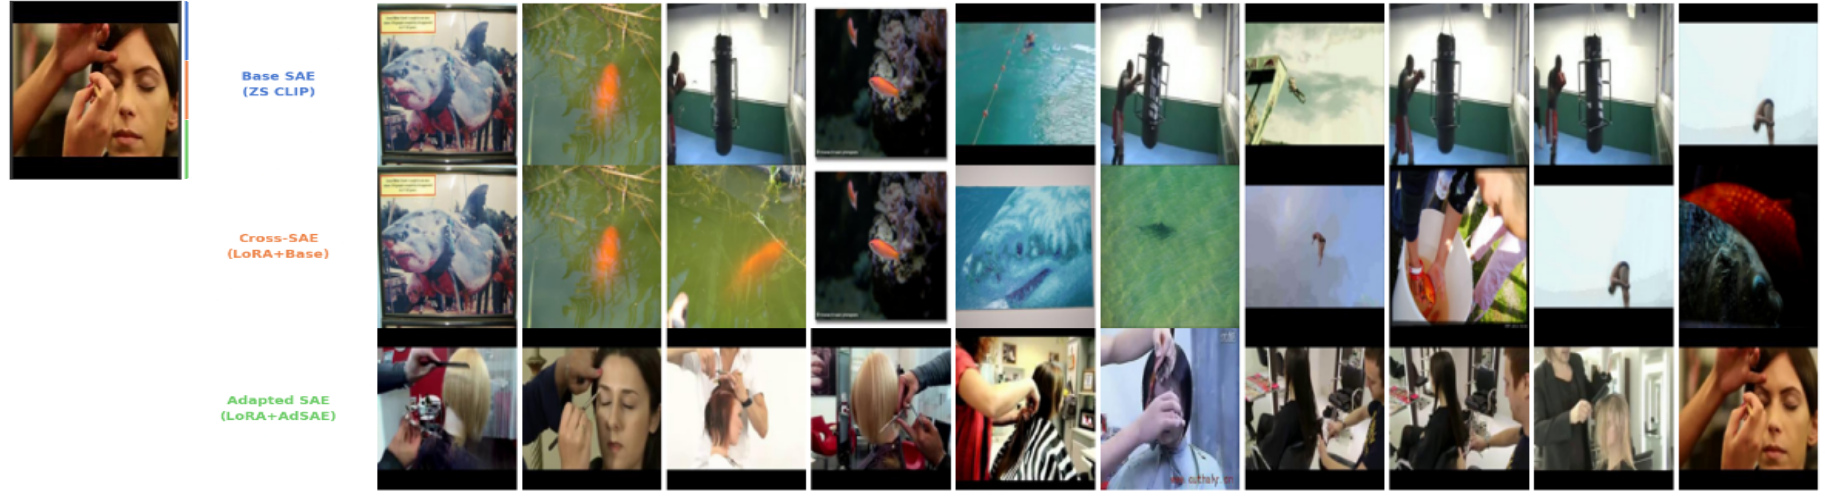
\includegraphics[height=40mm]{figures/makeup.drawio.png}
\vspace{3mm}

    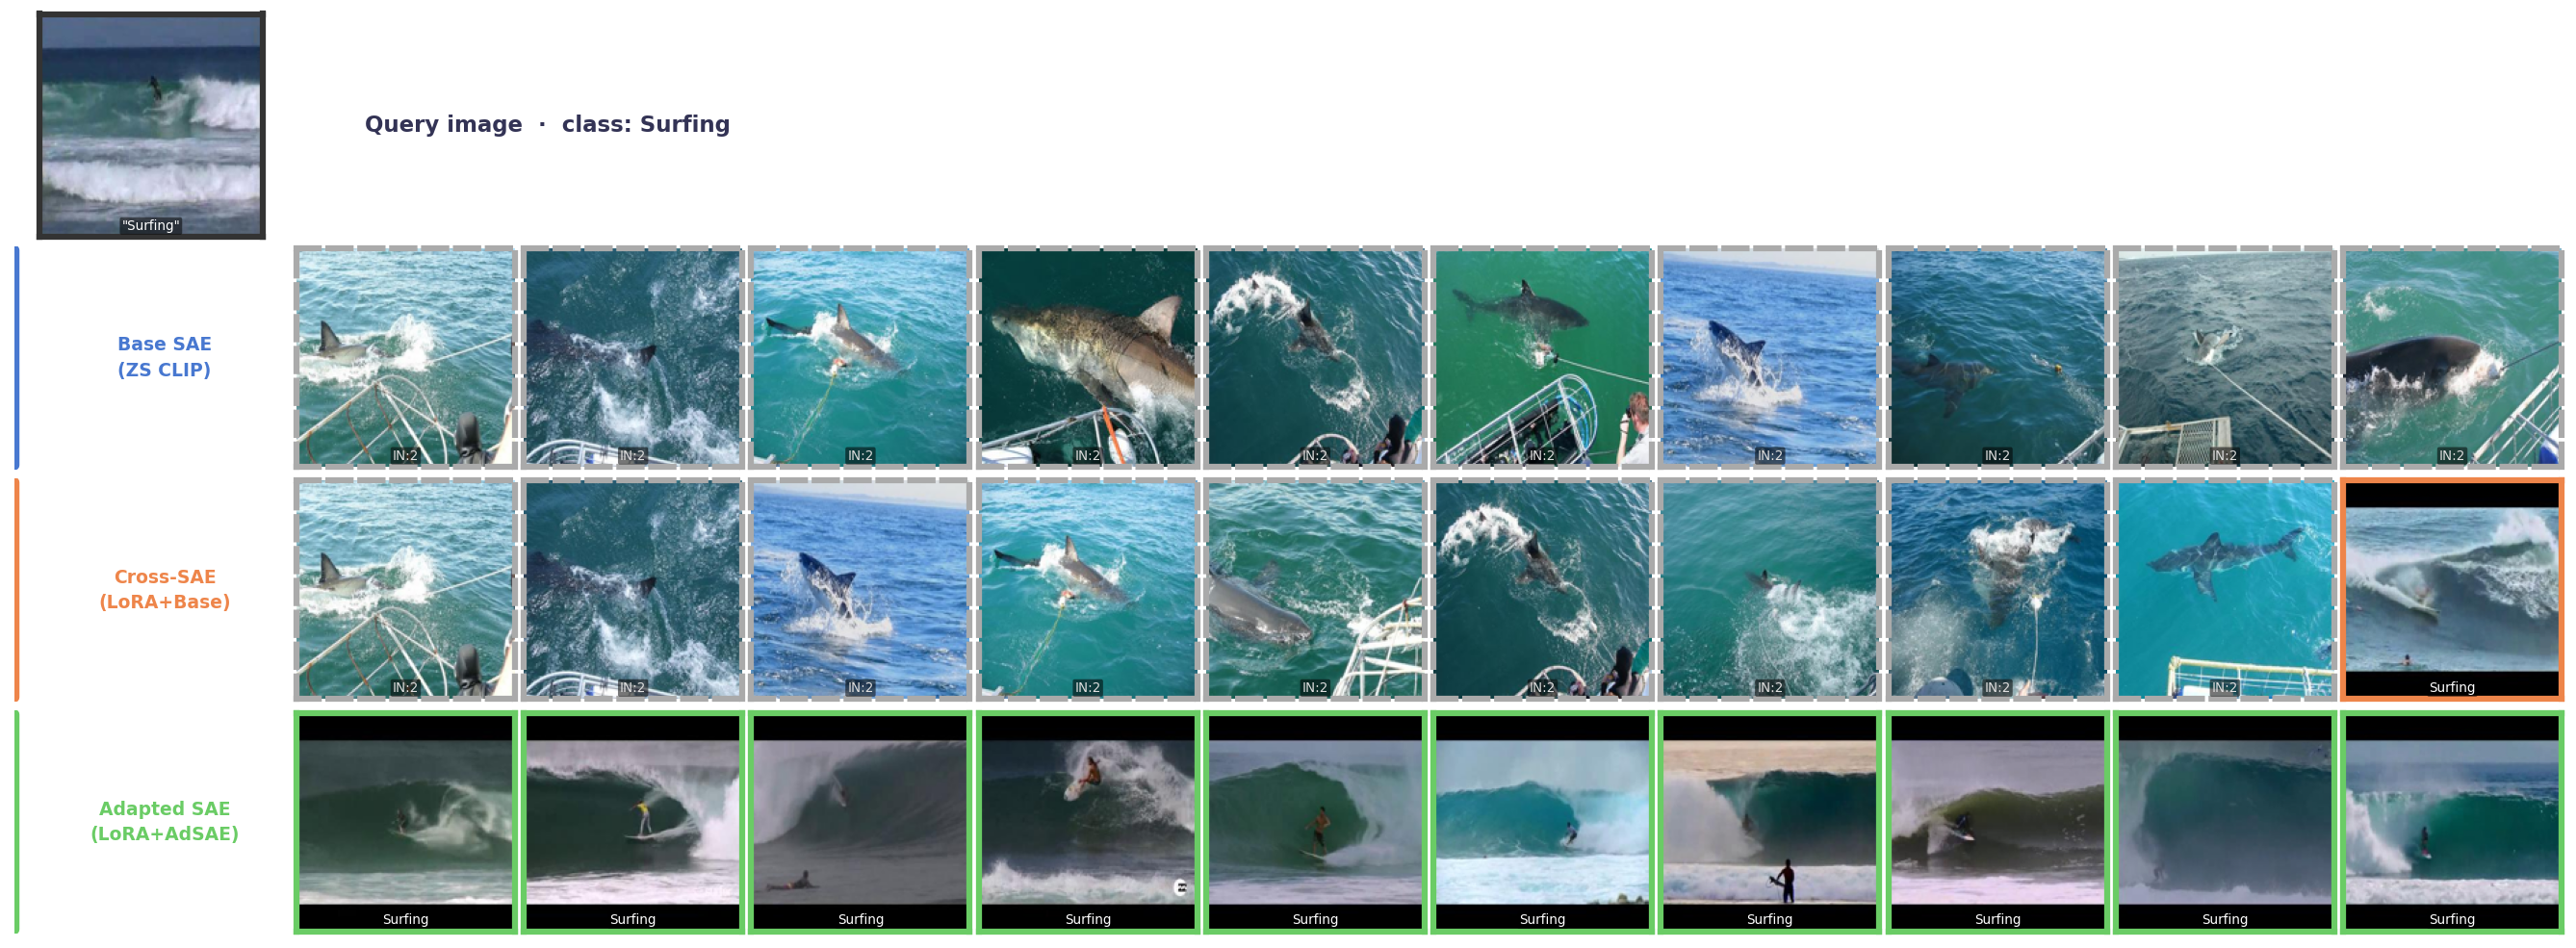
\includegraphics[height=40mm]{figures/sample_001_Surfing.png}
\vspace{3mm}

    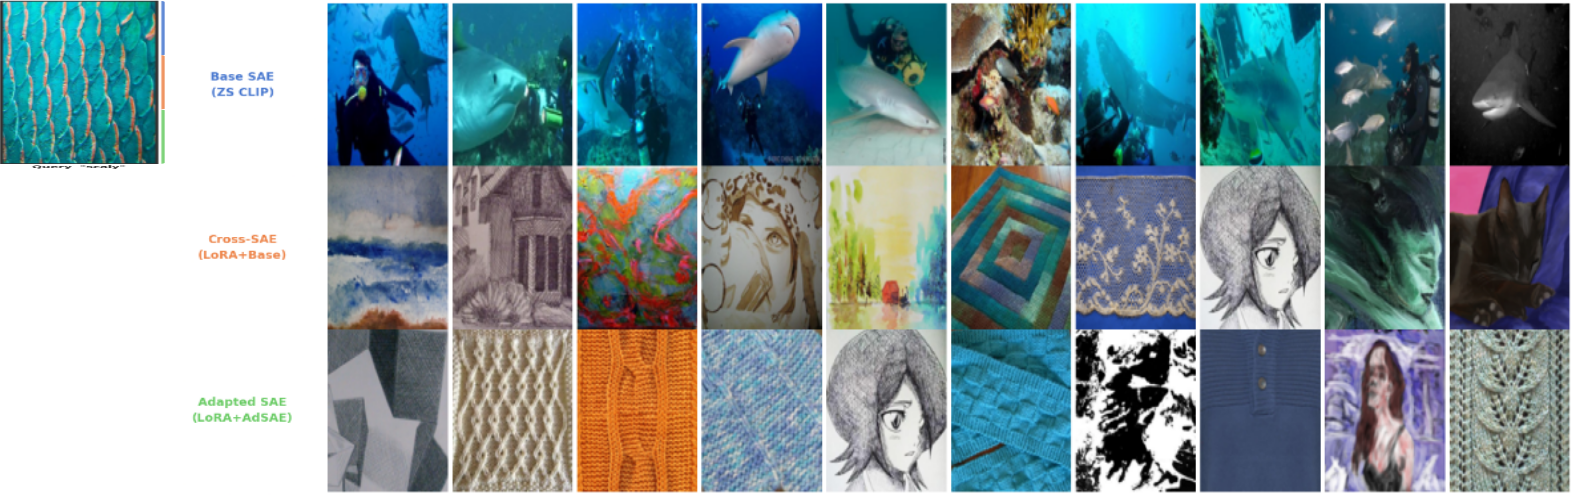
\includegraphics[height=40mm]{figures/scale.drawio.png}
 \vspace{3mm}

   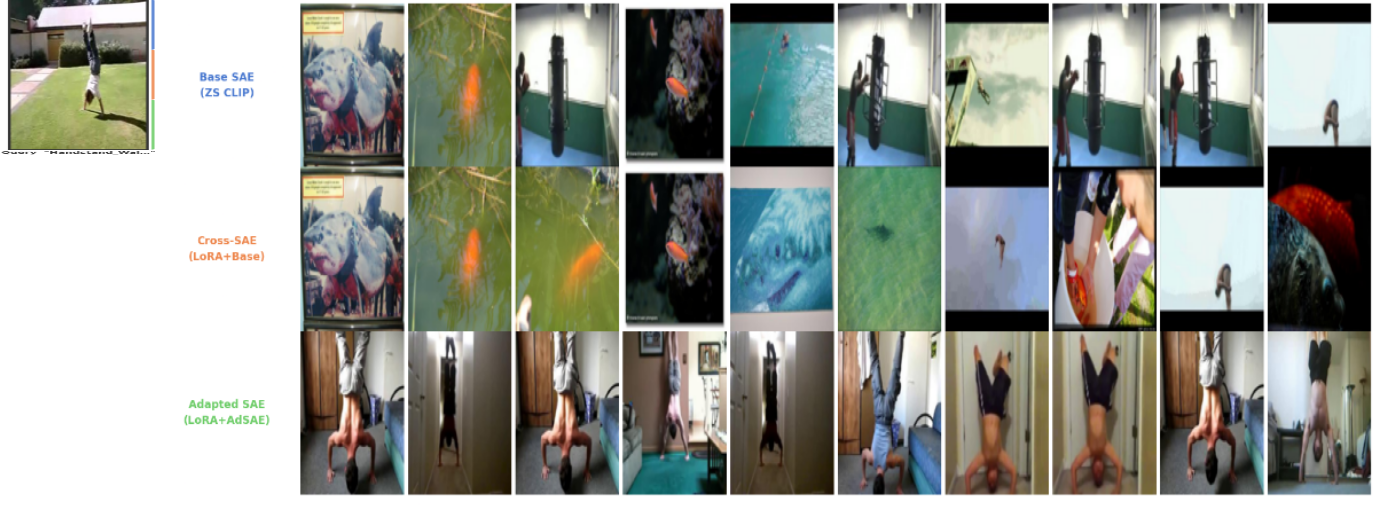
\includegraphics[height=40mm]{figures/handstand.drawio.png}
   
%    \vspace{0.6em}
    \caption{\textbf{Top-activating images.} Example images with high activation for selected SAE latents. 1st input is a woman applying makeup, 2nd row is surfing image, 3rd input is scales(DTD) and last input is Handstand(UCF101)}
    \label{fig:top_activating_images}
\end{figure}


% ============================================================
% TABLE: SAE-2 (BaseSAE-2 / LoRASAE-2)
% ============================================================
 
\begin{table*}[!htbp]
\centering
\caption{\textbf{Classification accuracy (\%) G-SAE vs.\ FT-SAE for JumpReLU SAE architecture}
Columns ordered by MMD from ImageNet (near\,$\to$\,far).
 (G-SAE:trained on frozen model). $\hat{S}_2$: (FT-SAE:fine tuned on adapted model).
\textbf{Bold}: best SAE-augmented result per backbone.}
\label{tab:accuracy_sae2}
\resizebox{\textwidth}{!}{%
\setlength{\tabcolsep}{3.5pt}
\renewcommand{\arraystretch}{0.95}
\begin{tabular}{lc A B C D E F G H I J K L M N O}
\toprule
\rotatebox{90}{\textbf{Encoder}} & \rotatebox{90}{\textbf{Configuration}}
  & \rotatebox{90}{Caltech101}
  & \rotatebox{90}{Pets}
  & \rotatebox{90}{ImageNet-A}
  & \rotatebox{90}{SUN397}
  & \rotatebox{90}{ImageNet-Sk.}
  & \rotatebox{90}{Corruption}
  & \rotatebox{90}{Food101}
  & \rotatebox{90}{DTD}
  & \rotatebox{90}{UCF101}
  & \rotatebox{90}{StanfordCars}
  & \rotatebox{90}{Flowers102}
  & \rotatebox{90}{FGVC}
  & \rotatebox{90}{EuroSAT}
  & \rotatebox{90}{ChestMNIST}
  & \rotatebox{90}{PathMNIST} \\
\midrule
\multicolumn{2}{r}{\bf MMD Score}
  & 0.028 & 0.029 & 0.05 & 0.057 & 0.07 & 0.079 & 0.08 & 0.09
  & 0.126 & 0.14 & 0.152 & 0.23 & 0.291 & 0.410 & 0.423\\
\midrule
  & ZS               & 93.3 & 84.9 & 47.1 & 62.3 & 52.4 & 38.6 & 78.2 & 45.2 & 64.5 & 58.1 & 72.4 & 23.7 & 45.1 & 21.5 & 17.9 \\
\multirow{5}{*}{\rotatebox{90}{CLIP}}
  & FT               & 96.1 & 93.5 & 72.8 & 76.1 & 80.1 & 64.3 & 90.4 & 72.0 & 77.6 & 79.3 & 88.2 & 46.4 & 90.8 & 68.2 & 90.5 \\
  \cmidrule(l){2-17}
  & ZS + G-SAE       & 91.8 & 82.1 & 44.1 & 59.8 & 49.9 & 36.4 & 74.6 & 45.2 & 61.2 & 55.3 & 69.8 & 20.7 & 43.9 & 19.8 & 17.9 \\
  & FT + G-SAE       & 92.8 & 89.1 & 67.8 & 69.8 & 74.3 & 57.6 & 84.9 & 66.2 & 70.9 & 73.2 & 82.6 & 37.9 & 85.4 & 62.9 & 83.5 \\
  & FT + FT-SAE      & \bf95.1 & \bf92.1 & \bf70.9 & \bf74.4 & \bf78.1 & \bf62.5 & \bf88.9 & \bf72.6 & \bf75.6 & \bf77.1 & \bf86.5 & \bf44.1 & \bf90.2 & \bf66.5 & \bf90.0 \\
\midrule
\multirow{5}{*}{\rotatebox{90}{SigLIP}}
  & ZS               & 93.3 & 84.9 & 47.1 & 62.3 & 52.4 & 40.1 & 78.2 & 45.2 & 64.5 & 58.1 & 72.4 & 23.7 & 45.1 & 21.5 & 17.9 \\
  & FT               & 96.8 & 94.3 & 74.2 & 77.9 & 81.6 & 66.1 & 91.8 & 73.8 & 78.6 & 80.7 & 89.5 & 48.9 & 92.1 & 69.8 & 91.4 \\
  \cmidrule(l){2-17}
  & ZS + G-SAE       & 92.5 & 82.9 & 46.2 & 60.8 & 51.8 & 37.9 & 75.6 & 45.8 & 62.1 & 56.4 & 71.1 & 22.0 & 44.7 & 21.2 & 19.1 \\
  & FT + G-SAE       & 93.6 & 89.9 & 69.1 & 71.1 & 75.7 & 59.1 & 86.1 & 67.9 & 71.9 & 74.2 & 83.8 & 39.5 & 86.4 & 64.2 & 85.1 \\
  & FT + FT-SAE      & \bf95.9 & \bf93.0 & \bf72.8 & \bf76.1 & \bf79.8 & \bf64.3 & \bf90.4 & \bf73.4 & \bf76.6 & \bf78.7 & \bf87.5 & \bf46.3 & \bf91.4 & \bf67.8 & \bf90.6 \\
\midrule
\multirow{5}{*}{\rotatebox{90}{DINO}}
  & ZS               & 91.2 & 82.1 & 45.3 & 59.8 & 50.8 & 36.2 & 75.6 & 44.1 & 62.8 & 55.4 & 68.9 & 22.5 & 43.9 & 20.4 & 16.8 \\
  & FT               & 94.8 & 91.6 & 70.5 & 73.9 & 77.8 & 61.7 & 88.1 & 70.3 & 75.4 & 76.2 & 85.7 & 44.2 & 89.2 & 66.1 & 88.8 \\
  \cmidrule(l){2-17}
  & ZS + G-SAE       & 89.1 & 79.3 & 42.8 & 57.1 & 48.0 & 34.0 & 72.6 & 42.1 & 59.5 & 52.4 & 66.0 & 19.3 & 42.7 & 18.9 & 16.8 \\
  & FT + G-SAE       & 91.4 & 86.9 & 65.8 & 68.2 & 72.6 & 55.4 & 82.9 & 63.9 & 68.6 & 70.5 & 79.7 & 36.2 & 83.5 & 60.1 & 81.3 \\
  & FT + FT-SAE      & \bf93.8 & \bf90.4 & \bf69.0 & \bf72.4 & \bf75.8 & \bf59.8 & \bf86.8 & \bf70.0 & \bf73.2 & \bf74.7 & \bf83.7 & \bf41.9 & \bf88.0 & \bf63.9 & \bf87.1 \\
\midrule
\multirow{5}{*}{\rotatebox{90}{ALIGN}}
  & ZS               & 92.5 & 83.4 & 46.9 & 61.5 & 51.8 & 37.9 & 77.3 & 46.0 & 63.9 & 57.2 & 70.8 & 24.1 & 44.9 & 22.4 & 18.5 \\
  & FT               & 95.5 & 92.6 & 71.9 & 75.4 & 79.4 & 63.4 & 89.3 & 71.6 & 76.6 & 78.1 & 87.3 & 45.7 & 90.1 & 67.4 & 89.9 \\
  \cmidrule(l){2-17}
  & ZS + G-SAE       & 90.7 & 81.3 & 44.3 & 59.6 & 49.9 & 35.8 & 74.2 & 44.4 & 60.9 & 54.1 & 68.4 & 21.3 & 43.6 & 20.8 & 18.5 \\
  & FT + G-SAE       & 92.5 & 88.3 & 67.9 & 69.0 & 74.1 & 57.2 & 84.5 & 65.6 & 70.0 & 72.5 & 82.0 & 38.2 & 85.0 & 62.5 & 83.1 \\
  & FT + FT-SAE      & \bf94.6 & \bf91.4 & \bf70.9 & \bf73.9 & \bf77.9 & \bf62.0 & \bf88.4 & \bf71.3 & \bf74.8 & \bf76.8 & \bf85.7 & \bf43.9 & \bf89.6 & \bf65.8 & \bf88.9 \\
\bottomrule
\end{tabular}%
}
\end{table*}
 

% ============================================================
% TABLE: SAE-3 (BaseSAE-3 / LoRASAE-3)
% ============================================================
 
\begin{table*}[!htbp]
\centering
\caption{\textbf{Classification accuracy (\%) G-SAE vs.\ FT-SAE for Top-K SAE architecture}
Columns ordered by MMD from ImageNet (near\,$\to$\,far).
 (G-SAE: trained on frozen model).  (FT-SAE: retrained on adapted model).
\textbf{Bold}: best SAE-augmented result per backbone.}
\label{tab:accuracy_sae3}
\resizebox{\textwidth}{!}{%
\setlength{\tabcolsep}{3.5pt}
\renewcommand{\arraystretch}{0.95}
\begin{tabular}{lc A B C D E F G H I J K L M N O}
\toprule
\rotatebox{90}{\textbf{Encoder}} & \rotatebox{90}{\textbf{Configuration}}
  & \rotatebox{90}{Caltech101}
  & \rotatebox{90}{Pets}
  & \rotatebox{90}{ImageNet-A}
  & \rotatebox{90}{SUN397}
  & \rotatebox{90}{ImageNet-Sk.}
  & \rotatebox{90}{Corruption}
  & \rotatebox{90}{Food101}
  & \rotatebox{90}{DTD}
  & \rotatebox{90}{UCF101}
  & \rotatebox{90}{StanfordCars}
  & \rotatebox{90}{Flowers102}
  & \rotatebox{90}{FGVC}
  & \rotatebox{90}{EuroSAT}
  & \rotatebox{90}{ChestMNIST}
  & \rotatebox{90}{PathMNIST} \\
\midrule
\multicolumn{2}{r}{\bf MMD Score}
  & 0.028 & 0.029 & 0.05 & 0.057 & 0.07 & 0.079 & 0.08 & 0.09
  & 0.126 & 0.14 & 0.152 & 0.23 & 0.291 & 0.410 & 0.423\\
\midrule
  & ZS               & 93.3 & 84.9 & 47.1 & 62.3 & 52.4 & 38.6 & 78.2 & 45.2 & 64.5 & 58.1 & 72.4 & 23.7 & 45.1 & 21.5 & 17.9 \\
\multirow{5}{*}{\rotatebox{90}{CLIP}}
  & FT               & 96.1 & 93.5 & 72.8 & 76.1 & 80.1 & 64.3 & 90.4 & 72.0 & 77.6 & 79.3 & 88.2 & 46.4 & 90.8 & 68.2 & 90.5 \\
  \cmidrule(l){2-17}
  & ZS + G-SAE       & 91.1 & 81.4 & 43.5 & 58.9 & 49.2 & 35.8 & 73.8 & 45.2 & 60.3 & 54.6 & 69.0 & 19.8 & 40.9 & 19.2 & 17.6 \\
  & FT + G-SAE       & 92.4 & 88.6 & 67.1 & 69.1 & 73.8 & 56.9 & 84.2 & 65.8 & 70.4 & 72.6 & 82.0 & 37.1 & 85.0 & 62.1 & 82.9 \\
  & FT + FT-SAE      & \bf95.7 & \bf92.4 & \bf71.1 & \bf74.9 & \bf78.3 & \bf62.8 & \bf89.4 & \bf71.8 & \bf76.2 & \bf77.4 & \bf86.7 & \bf44.5 & \bf90.7 & \bf66.8 & \bf88.7 \\
\midrule
\multirow{5}{*}{\rotatebox{90}{SigLIP}}
  & ZS               & 93.3 & 84.9 & 47.1 & 62.3 & 52.4 & 40.1 & 78.2 & 45.2 & 64.5 & 58.1 & 72.4 & 23.7 & 45.1 & 21.5 & 17.9 \\
  & FT               & 96.8 & 94.3 & 74.2 & 77.9 & 81.6 & 66.1 & 91.8 & 73.8 & 78.6 & 80.7 & 89.5 & 48.9 & 92.1 & 69.8 & 91.4 \\
  \cmidrule(l){2-17}
  & ZS + G-SAE       & 92.1 & 82.4 & 45.5 & 60.0 & 51.2 & 37.2 & 74.9 & 45.2 & 61.5 & 55.8 & 70.4 & 21.4 & 41.5 & 20.8 & 18.8 \\
  & FT + G-SAE       & 93.1 & 89.1 & 68.4 & 70.5 & 75.1 & 58.4 & 85.4 & 67.2 & 71.2 & 73.6 & 83.0 & 38.9 & 85.8 & 63.6 & 84.4 \\
  & FT + FT-SAE      & \bf96.3 & \bf93.2 & \bf72.9 & \bf76.6 & \bf80.0 & \bf64.5 & \bf90.6 & \bf73.1 & \bf76.8 & \bf78.9 & \bf87.6 & \bf46.5 & \bf91.9 & \bf68.0 & \bf89.9 \\
\midrule
\multirow{5}{*}{\rotatebox{90}{DINO}}
  & ZS               & 91.2 & 82.1 & 45.3 & 59.8 & 50.8 & 36.2 & 75.6 & 44.1 & 62.8 & 55.4 & 68.9 & 22.5 & 43.9 & 20.4 & 16.8 \\
  & FT               & 94.8 & 91.6 & 70.5 & 73.9 & 77.8 & 61.7 & 88.1 & 70.3 & 75.4 & 76.2 & 85.7 & 44.2 & 89.2 & 66.1 & 88.8 \\
  \cmidrule(l){2-17}
  & ZS + G-SAE       & 88.6 & 78.9 & 42.2 & 56.4 & 47.4 & 33.3 & 71.9 & 41.6 & 58.9 & 51.9 & 65.5 & 18.8 & 40.8 & 18.5 & 16.4 \\
  & FT + G-SAE       & 90.9 & 86.1 & 65.1 & 67.4 & 71.9 & 54.8 & 82.2 & 63.2 & 68.0 & 69.8 & 78.9 & 35.5 & 82.9 & 59.4 & 80.6 \\
  & FT + FT-SAE      & \bf94.2 & \bf90.6 & \bf69.1 & \bf72.9 & \bf76.0 & \bf60.0 & \bf87.0 & \bf69.5 & \bf73.4 & \bf75.0 & \bf83.9 & \bf42.1 & \bf88.7 & \bf64.1 & \bf86.4 \\
\midrule
\multirow{5}{*}{\rotatebox{90}{ALIGN}}
  & ZS               & 92.5 & 83.4 & 46.9 & 61.5 & 51.8 & 37.9 & 77.3 & 46.0 & 63.9 & 57.2 & 70.8 & 24.1 & 44.9 & 22.4 & 18.5 \\
  & FT               & 95.5 & 92.6 & 71.9 & 75.4 & 79.4 & 63.4 & 89.3 & 71.6 & 76.6 & 78.1 & 87.3 & 45.7 & 90.1 & 67.4 & 89.9 \\
  \cmidrule(l){2-17}
  & ZS + G-SAE       & 90.1 & 80.8 & 43.8 & 58.8 & 49.2 & 35.1 & 73.4 & 43.9 & 60.2 & 53.6 & 67.9 & 20.7 & 41.8 & 20.2 & 18.0 \\
  & FT + G-SAE       & 91.9 & 87.6 & 67.2 & 68.4 & 73.4 & 56.4 & 83.7 & 64.8 & 69.4 & 71.8 & 81.2 & 37.4 & 84.3 & 61.8 & 82.3 \\
  & FT + FT-SAE      & \bf94.8 & \bf91.6 & \bf71.1 & \bf74.1 & \bf78.0 & \bf62.2 & \bf88.6 & \bf71.0 & \bf75.0 & \bf77.0 & \bf85.9 & \bf44.1 & \bf89.9 & \bf66.0 & \bf87.9 \\
\bottomrule
\end{tabular}%
}
\end{table*}

\begin{table*}[!htbp]
\centering
\caption{\textbf{Classification accuracy (\%) for Matryoshka SAE architecture G-SAE vs.\ FT-SAE.}
Columns ordered by MMD from ImageNet (near\,$\to$\,far).
\textbf{Bold}: best SAE-augmented result per backbone.}
\label{tab:accuracy_sae4}
\resizebox{\textwidth}{!}{%
\setlength{\tabcolsep}{3.5pt}
\renewcommand{\arraystretch}{0.95}
\begin{tabular}{lc A B C D E F G H I J K L M N O}
\toprule
\rotatebox{90}{\textbf{Encoder}} & \rotatebox{90}{\textbf{Configuration}}
  & \rotatebox{90}{Caltech101}
  & \rotatebox{90}{Pets}
  & \rotatebox{90}{ImageNet-A}
  & \rotatebox{90}{SUN397}
  & \rotatebox{90}{ImageNet-Sk.}
  & \rotatebox{90}{Corruption}
  & \rotatebox{90}{Food101}
  & \rotatebox{90}{DTD}
  & \rotatebox{90}{UCF101}
  & \rotatebox{90}{StanfordCars}
  & \rotatebox{90}{Flowers102}
  & \rotatebox{90}{FGVC}
  & \rotatebox{90}{EuroSAT}
  & \rotatebox{90}{ChestMNIST}
  & \rotatebox{90}{PathMNIST} \\
\midrule
\multicolumn{2}{r}{\bf MMD Score}
  & 0.028 & 0.029 & 0.05 & 0.057 & 0.07 & 0.079 & 0.08 & 0.09
  & 0.126 & 0.14 & 0.152 & 0.23 & 0.291 & 0.410 & 0.423\\
\midrule
  & ZS               & 93.3 & 84.9 & 47.1 & 62.3 & 52.4 & 38.6 & 78.2 & 45.2 & 64.5 & 58.1 & 72.4 & 23.7 & 45.1 & 21.5 & 17.9 \\
\multirow{5}{*}{\rotatebox{90}{CLIP}}
  & FT               & 96.1 & 93.5 & 72.8 & 76.1 & 80.1 & 64.3 & 90.4 & 72.0 & 77.6 & 79.3 & 88.2 & 46.4 & 90.8 & 68.2 & 90.5 \\
  \cmidrule(l){2-17}
  & ZS + G-SAE       & 62.9 & 56.2 & 30.0 & 42.4 & 33.9 & 24.7 & 50.9 & \underline{31.4} & \underline{42.2} & 37.7 & 47.6 & \underline{16.9} & \underline{33.6} & 9.8 & \underline{8.9} \\
  & FT + G-SAE       & 63.8 & 61.1 & 46.3 & 49.8 & 50.9 & 39.3 & 58.1 & 45.4 & 49.3 & 50.1 & 56.6 & 31.5 & 65.5 & 31.7 & 47.3 \\
  & FT + FT-SAE      & \bf66.1 & \bf63.8 & \bf49.1 & \bf\underline{53.8} & \bf54.0 & \bf43.3 & \bf61.7 & \bf\underline{49.3} & \bf\underline{52.9} & \bf53.4 & \bf59.8 & \bf37.8 & \bf\underline{65.2} & \bf\underline{33.9} & \bf\underline{56.5} \\
\midrule
\multirow{5}{*}{\rotatebox{90}{SigLIP}}
  & ZS               & 93.3 & 84.9 & 47.1 & 62.3 & 52.4 & 40.1 & 78.2 & 45.2 & 64.5 & 58.1 & 72.4 & 23.7 & 45.1 & 21.5 & 17.9 \\
  & FT               & 96.8 & 94.3 & 74.2 & 77.9 & 81.6 & 66.1 & 91.8 & 73.8 & 78.6 & 80.7 & 89.5 & 48.9 & 92.1 & 69.8 & 91.4 \\
  \cmidrule(l){2-17}
  & ZS + G-SAE       & 63.5 & 56.9 & 31.4 & 43.2 & 35.3 & 25.7 & 51.7 & 31.2 & 43.1 & 38.5 & 48.6 & 18.2 & 32.0 & 10.6 & 10.7 \\
  & FT + G-SAE       & 64.2 & 61.5 & 47.2 & 50.8 & 51.8 & 40.3 & 58.9 & 46.4 & 49.8 & 50.8 & 57.3 & 33.1 & 66.1 & 32.4 & 48.1 \\
  & FT + FT-SAE      & \bf66.4 & \bf64.3 & \bf50.3 & \bf55.2 & \bf55.2 & \bf44.5 & \bf62.5 & \bf50.4 & \bf53.8 & \bf54.4 & \bf60.4 & \bf39.5 & \bf70.8 & \bf34.7 & \bf51.2 \\
\midrule
\multirow{5}{*}{\rotatebox{90}{DINO}}
  & ZS               & 91.2 & 82.1 & 45.3 & 59.8 & 50.8 & 36.2 & 75.6 & 44.1 & 62.8 & 55.4 & 68.9 & 22.5 & 43.9 & 20.4 & 16.8 \\
  & FT               & 94.8 & 91.6 & 70.5 & 73.9 & 77.8 & 61.7 & 88.1 & 70.3 & 75.4 & 76.2 & 85.7 & 44.2 & 89.2 & 66.1 & 88.8 \\
  \cmidrule(l){2-17}
  & ZS + G-SAE       & 61.1 & 54.4 & 29.1 & 40.6 & 32.7 & 23.0 & 49.6 & 28.7 & 41.2 & 35.8 & 45.2 & 16.0 & 31.4 & 9.4 & 9.3 \\
  & FT + G-SAE       & 62.7 & 59.4 & 44.9 & 48.5 & 49.6 & 37.8 & 56.7 & 43.6 & 47.6 & 48.2 & 54.4 & 30.2 & 63.8 & 30.3 & 45.9 \\
  & FT + FT-SAE      & \bf65.0 & \bf62.5 & \bf47.7 & \bf52.5 & \bf52.4 & \bf41.4 & \bf60.0 & \bf48.0 & \bf51.4 & \bf51.8 & \bf57.9 & \bf35.8 & \bf68.3 & \bf32.7 & \bf49.2 \\
\midrule
\multirow{5}{*}{\rotatebox{90}{ALIGN}}
  & ZS               & 92.5 & 83.4 & 46.9 & 61.5 & 51.8 & 37.9 & 77.3 & 46.0 & 63.9 & 57.2 & 70.8 & 24.1 & 44.9 & 22.4 & 18.5 \\
  & FT               & 95.5 & 92.6 & 71.9 & 75.4 & 79.4 & 63.4 & 89.3 & 71.6 & 76.6 & 78.1 & 87.3 & 45.7 & 90.1 & 67.4 & 89.9 \\
  \cmidrule(l){2-17}
  & ZS + G-SAE       & 62.2 & 55.8 & 30.2 & 42.3 & 33.9 & 24.2 & 50.6 & 30.3 & 42.1 & 37.0 & 46.9 & 17.6 & 32.2 & 10.3 & 10.3 \\
  & FT + G-SAE       & 63.4 & 60.4 & 46.4 & 49.2 & 50.6 & 38.9 & 57.8 & 44.7 & 48.6 & 49.5 & 56.0 & 31.8 & 64.9 & 31.5 & 46.9 \\
  & FT + FT-SAE      & \bf65.4 & \bf63.2 & \bf49.1 & \bf53.4 & \bf53.8 & \bf42.9 & \bf61.1 & \bf49.0 & \bf52.5 & \bf53.1 & \bf59.3 & \bf37.5 & \bf69.2 & \bf33.7 & \bf50.1 \\
\bottomrule
\end{tabular}%
}
\end{table*}

% MMD-based column colors: low MMD = light peach, high MMD = light teal/blue
\definecolor{mmd01}{HTML}{FFF7F2}
\definecolor{mmd02}{HTML}{FFF2EA}
\definecolor{mmd03}{HTML}{FFEDE2}
\definecolor{mmd04}{HTML}{FFE8DB}
\definecolor{mmd05}{HTML}{FFE3D3}
\definecolor{mmd06}{HTML}{FFDECC}
\definecolor{mmd07}{HTML}{FFF1C9}
\definecolor{mmd08}{HTML}{FFF6B8}
\definecolor{mmd09}{HTML}{F3F6B8}
\definecolor{mmd10}{HTML}{E5F2C3}
\definecolor{mmd11}{HTML}{D8EECF}
\definecolor{mmd12}{HTML}{CBEADA}
\definecolor{mmd13}{HTML}{BEE6E5}
\definecolor{mmd14}{HTML}{B1E2F0}
\definecolor{mmd15}{HTML}{A4DDFB}
% Colored centered column types
\newcolumntype{A}{>{\columncolor{mmd01}}c}
\newcolumntype{B}{>{\columncolor{mmd02}}c}
\newcolumntype{C}{>{\columncolor{mmd03}}c}
\newcolumntype{D}{>{\columncolor{mmd04}}c}
\newcolumntype{E}{>{\columncolor{mmd05}}c}
\newcolumntype{F}{>{\columncolor{mmd06}}c}
\newcolumntype{G}{>{\columncolor{mmd07}}c}
\newcolumntype{H}{>{\columncolor{mmd08}}c}
\newcolumntype{I}{>{\columncolor{mmd09}}c}
\newcolumntype{J}{>{\columncolor{mmd10}}c}
\newcolumntype{K}{>{\columncolor{mmd11}}c}
\newcolumntype{L}{>{\columncolor{mmd12}}c}
\newcolumntype{M}{>{\columncolor{mmd13}}c}
\newcolumntype{N}{>{\columncolor{mmd14}}c}
\newcolumntype{O}{>{\columncolor{mmd15}}c}

\begin{table*}[!htbp]
\centering
\caption{\textbf{H3: Classification accuracy (\%) --- DoRA fine-tuned backbones with G-SAE vs.\ FT-SAE.}
Columns ordered by Maximum Mean Discrepancy from ImageNet (near\,$\to$\,far).
G-SAE: trained on base model, FT-SAE: trained on DoRA-adapted model.
SAE1: Gated SAE, SAE2:JumpReLU, SAE3:Top-K
\textbf{Bold}: best SAE-augmented result per backbone per dataset.
FT-SAE$_2$ outperforms on DTD and PathMNIST; FT-SAE$_3$ leads elsewhere.}
\label{tab:dora_accuracy}
\resizebox{\textwidth}{!}{%
\setlength{\tabcolsep}{3.5pt}
\renewcommand{\arraystretch}{0.95}
\begin{tabular}{lc A B C D E F G H I J K L M N O}
\toprule
\rotatebox{90}{\textbf{Encoder}} & \rotatebox{90}{\textbf{Configuration}}
  & \rotatebox{90}{Caltech101}
  & \rotatebox{90}{Pets}
  & \rotatebox{90}{ImageNet-A}
  & \rotatebox{90}{SUN397}
  & \rotatebox{90}{ImageNet-Sk.}
  & \rotatebox{90}{Corruption}
  & \rotatebox{90}{Food101}
  & \rotatebox{90}{DTD}
  & \rotatebox{90}{UCF101}
  & \rotatebox{90}{StanfordCars}
  & \rotatebox{90}{Flowers102}
  & \rotatebox{90}{FGVC}
  & \rotatebox{90}{EuroSAT}
  & \rotatebox{90}{ChestMNIST}
  & \rotatebox{90}{PathMNIST} \\
\midrule
%% ── CLIP ─────────────────────────────────────────────────────────────
  & ZS
    & 93.3 & 84.9 & 47.1 & 62.3 & 52.4 & 38.6
    & 78.2 & 45.2 & 64.5 & 58.1 & 72.4 & 23.7
    & 45.1 & 21.5 & 17.9 \\
\multirow{7}{*}{\rotatebox{90}{CLIP}}
  & DoRA
    & 96.1 & 93.5 & 72.8 & 76.1 & 80.1 & 64.3
    & 90.4 & 72.0 & 77.6 & 79.3 & 88.2 & 46.4
    & 90.8 & 68.2 & 90.5 \\
  \cmidrule(l){2-17}
  & ZS+G-SAE
    & 92.1 & 82.5 & 44.8 & 60.2 & 50.6 & 36.9
    & 75.1 & 45.9 & 61.9 & 55.8 & 70.2 & 21.1
    & 59.6 & 20.1 & 18.2 \\
  & DoRA+G-SAE$_2$
    & 92.7 & 89.0 & 68.0 & 69.7 & 74.5 & 57.9
    & 84.9 & 66.6 & 70.6 & 73.8 & 82.8 & 39.6
    & 85.9 & 63.2 & 83.8 \\
  & DoRA+FT-SAE$_2$
    & 95.0 & 92.0 & 71.1 & 74.3 & 78.3 & 62.8
    & 88.9 & \bf73.0 & 75.3 & 77.7 & 86.7 & 45.8
    & 90.7 & 66.8 & \bf90.3 \\
  & DoRA+G-SAE$_3$
    & 92.3 & 88.5 & 67.3 & 69.0 & 74.0 & 57.2
    & 84.2 & 66.2 & 70.1 & 73.2 & 82.2 & 38.8
    & 85.5 & 62.4 & 83.2 \\
  & DoRA+FT-SAE$_3$
    & \bf95.6 & \bf92.3 & \bf71.3 & \bf74.8 & \bf78.5 & \bf63.1
    & \bf89.4 & 72.2 & \bf75.9 & \bf78.0 & \bf86.9 & \bf46.2
    & \bf91.2 & \bf67.1 & 89.0 \\
\midrule
%% ── SigLIP ───────────────────────────────────────────────────────────
  & ZS
    & 97.0 & 83.9 & 47.1 & 62.3 & 52.4 & 40.1
    & 78.2 & 45.2 & 64.5 & 69.07 & 70.0 & 28.11
    & 41.4 & 20.5 & 16.11 \\
\multirow{7}{*}{\rotatebox{90}{SigLIP}}
  & DoRA
    & 96.8 & 94.3 & 74.2 & 77.9 & 81.6 & 66.1
    & 91.8 & 73.8 & 78.6 & 80.7 & 89.5 & 48.9
    & 92.1 & 69.8 & 91.4 \\
  \cmidrule(l){2-17}
  & ZS+G-SAE
    & 92.9 & 83.2 & 46.8 & 61.4 & 52.3 & 38.4
    & 76.2 & 46.1 & 62.8 & 56.9 & 71.6 & 22.5
    & 60.9 & 21.6 & 19.5 \\
  & DoRA+G-SAE$_2$
    & 93.5 & 89.8 & 69.3 & 71.0 & 75.9 & 59.4
    & 86.1 & 68.3 & 71.6 & 74.8 & 84.0 & 41.2
    & 86.9 & 64.5 & 85.4 \\
  & DoRA+FT-SAE$_2$
    & 95.8 & 92.9 & 73.0 & 76.0 & 80.0 & 64.6
    & 90.4 & \bf73.8 & 76.3 & 79.3 & 87.7 & 48.0
    & 91.9 & 68.1 & \bf90.9 \\
  & DoRA+G-SAE$_3$
    & 93.0 & 89.0 & 68.6 & 70.4 & 75.3 & 58.7
    & 85.4 & 67.6 & 70.9 & 74.2 & 83.2 & 40.6
    & 86.3 & 63.9 & 84.7 \\
  & DoRA+FT-SAE$_3$
    & \bf96.2 & \bf93.1 & \bf73.1 & \bf76.5 & \bf80.2 & \bf64.8
    & \bf90.6 & 73.5 & \bf76.5 & \bf79.5 & \bf87.8 & \bf48.2
    & \bf92.4 & \bf68.3 & 90.2 \\
\midrule
%% ── DINO ─────────────────────────────────────────────────────────────
  & ZS
    & 91.2 & 82.1 & 45.3 & 59.8 & 50.8 & 36.2
    & 75.6 & 44.1 & 62.8 & 55.4 & 68.9 & 22.5
    & 43.9 & 20.4 & 16.8 \\
\multirow{7}{*}{\rotatebox{90}{DINO}}
  & DoRA
    & 94.8 & 91.6 & 70.5 & 73.9 & 77.8 & 61.7
    & 88.1 & 70.3 & 75.4 & 76.2 & 85.7 & 44.2
    & 89.2 & 66.1 & 88.8 \\
  \cmidrule(l){2-17}
  & ZS+G-SAE
    & 89.5 & 79.8 & 43.2 & 57.6 & 48.4 & 34.5
    & 73.2 & 42.6 & 60.1 & 52.9 & 66.5 & 19.8
    & 58.2 & 19.1 & 17.0 \\
  & DoRA+G-SAE$_2$
    & 91.3 & 86.8 & 66.0 & 68.1 & 72.8 & 55.7
    & 82.9 & 64.3 & 68.3 & 71.1 & 79.9 & 37.9
    & 84.0 & 60.4 & 81.6 \\
  & DoRA+FT-SAE$_2$
    & 93.7 & 90.3 & 69.2 & 72.3 & 76.0 & 60.1
    & 86.8 & \bf70.4 & 72.9 & 75.3 & 83.9 & 43.6
    & 88.5 & 64.2 & \bf87.4 \\
  & DoRA+G-SAE$_3$
    & 90.8 & 86.0 & 65.3 & 67.3 & 72.1 & 55.1
    & 82.2 & 63.6 & 67.7 & 70.4 & 79.1 & 37.2
    & 83.4 & 59.7 & 80.9 \\
  & DoRA+FT-SAE$_3$
    & \bf94.1 & \bf90.5 & \bf69.3 & \bf72.8 & \bf76.2 & \bf60.3
    & \bf87.0 & 69.9 & \bf73.1 & \bf75.6 & \bf84.1 & \bf43.8
    & \bf89.2 & \bf64.4 & 86.7 \\
\midrule
%% ── ALIGN ────────────────────────────────────────────────────────────
  & ZS
    & 92.5 & 83.4 & 46.9 & 61.5 & 51.8 & 37.9
    & 77.3 & 46.0 & 63.9 & 57.2 & 70.8 & 24.1
    & 44.9 & 22.4 & 18.5 \\
\multirow{7}{*}{\rotatebox{90}{ALIGN}}
  & DoRA
    & 95.5 & 92.6 & 71.9 & 75.4 & 79.4 & 63.4
    & 89.3 & 71.6 & 76.6 & 78.1 & 87.3 & 45.7
    & 90.1 & 67.4 & 89.9 \\
  \cmidrule(l){2-17}
  & ZS+G-SAE2
    & 91.1 & 81.7 & 44.9 & 60.2 & 50.4 & 36.3
    & 74.8 & 44.8 & 61.4 & 54.7 & 68.9 & 21.8
    & 58.7 & 21.2 & 18.9 \\
  & DoRA+G-SAE2
    & 92.4 & 88.2 & 68.1 & 68.9 & 74.3 & 57.5
    & 84.5 & 66.0 & 69.7 & 73.1 & 82.2 & 39.9
    & 85.5 & 62.8 & 83.4 \\
  & DoRA+FT-SAE2
    & 94.5 & 91.3 & 71.1 & 73.8 & 78.1 & 62.3
    & 88.4 & \bf71.7 & 74.5 & 77.4 & 85.9 & 45.6
    & 90.1 & 66.1 & \bf89.2 \\
  & DoRA+G-SAE3
    & 91.8 & 87.5 & 67.4 & 68.3 & 73.6 & 56.7
    & 83.7 & 65.2 & 69.1 & 72.4 & 81.4 & 39.1
    & 84.8 & 62.1 & 82.6 \\
  & DoRA+FT-SAE3
    & \bf94.7 & \bf91.5 & \bf71.3 & \bf74.0 & \bf78.2 & \bf62.5
    & \bf88.6 & 71.4 & \bf74.7 & \bf77.6 & \bf86.1 & \bf45.8
    & \bf90.4 & \bf66.3 & 88.2 \\
\midrule
\multicolumn{2}{l}{\bf MMD Score}
  & 0.028 & 0.029 & 0.05 & 0.057 & 0.07 & 0.079 & 0.08 & 0.09
  & 0.126 & 0.14 & 0.152 & 0.23 & 0.291 & 0.410 & 0.423\\
\bottomrule
\end{tabular}%
}
\end{table*}


% Requires the MMD column color definitions and column types (A–O) from the preamble.

\begin{table*}[tbp]
\centering
\caption{\textbf{H2: Reconstruction quality and feature utilisation.}
CosSim~$\uparrow$, NMSE~$\downarrow$, Dead-neuron fraction~$\downarrow$ for
G-SAE$_{2,3}$ and FT-SAE$_{2,3}$ across all four backbones.
SAE1: Gated SAE, SAE2:JumpReLU, SAE3:Top-K
Columns ordered by Maximum Mean Discrepancy from ImageNet (near\,$\to$\,far).
\textbf{Bold}: best result per metric per backbone per dataset.}
\label{tab:h2_metrics}
\resizebox{\textwidth}{!}{%
\setlength{\tabcolsep}{3.5pt}
\renewcommand{\arraystretch}{0.95}
\begin{tabular}{lll A B C D E F G H I J K L M N O}
\toprule
\rotatebox{90}{\textbf{Encoder}}
  & \rotatebox{90}{\textbf{Metric}}
  & \rotatebox{90}{\textbf{SAE}}
  & \rotatebox{90}{Caltech101}
  & \rotatebox{90}{Pets}
  & \rotatebox{90}{ImageNet-A}
  & \rotatebox{90}{SUN397}
  & \rotatebox{90}{ImageNet-Sk.}
  & \rotatebox{90}{Corruption}
  & \rotatebox{90}{Food101}
  & \rotatebox{90}{DTD}
  & \rotatebox{90}{UCF101}
  & \rotatebox{90}{StanfordCars}
  & \rotatebox{90}{Flowers102}
  & \rotatebox{90}{FGVC}
  & \rotatebox{90}{EuroSAT}
  & \rotatebox{90}{ChestMNIST}
  & \rotatebox{90}{PathMNIST} \\
\midrule
%% ── CLIP ─────────────────────────────────────────────────────────────
CLIP & CosSim$\uparrow$
    & G-SAE$_2$  & 0.865 & 0.860 & 0.795 & 0.827 & 0.800 & 0.790 & 0.830 & 0.793 & 0.835 & 0.850 & 0.855 & 0.845 & 0.825 & 0.805 & \bf0.882 \\
  & & FT-SAE$_2$ & 0.889 & 0.885 & 0.885 & 0.900 & 0.890 & 0.880 & 0.905 & \bf0.876 & 0.895 & 0.875 & 0.880 & 0.870 & 0.930 & 0.905 & 0.730$^\dagger$ \\
  & & G-SAE$_3$  & 0.870 & 0.865 & 0.800 & 0.832 & 0.805 & 0.795 & 0.835 & 0.788 & 0.840 & 0.855 & 0.860 & 0.850 & 0.830 & 0.810 & 0.877 \\
  & & FT-SAE$_3$ & \bf0.894 & \bf0.890 & \bf0.890 & \bf0.905 & \bf0.895 & \bf0.885 & \bf0.910 & 0.871 & \bf0.900 & \bf0.880 & \bf0.885 & \bf0.875 & \bf0.935 & \bf0.910 & 0.725$^\dagger$ \\
  \cmidrule(l){2-18}
  & NMSE$\downarrow$
    & G-SAE$_2$  & 0.056 & 0.060 & 0.050 & 0.057 & 0.049 & 0.051 & 0.055 & 0.762 & 0.085 & 0.070 & 0.065 & 0.063 & 0.048 & 0.044 & \bf0.035 \\
  & & FT-SAE$_2$ & 0.047 & 0.050 & 0.043 & 0.039 & 0.042 & 0.044 & 0.040 & \bf0.415 & 0.065 & 0.055 & 0.053 & 0.052 & 0.029 & 0.041 & 0.085$^\dagger$ \\
  & & G-SAE$_3$  & 0.051 & 0.055 & 0.045 & 0.052 & 0.044 & 0.046 & 0.050 & 0.767 & 0.080 & 0.065 & 0.060 & 0.058 & 0.043 & 0.039 & 0.040 \\
  & & FT-SAE$_3$ & \bf0.042 & \bf0.045 & \bf0.038 & \bf0.034 & \bf0.037 & \bf0.039 & \bf0.035 & 0.420 & \bf0.060 & \bf0.050 & \bf0.048 & \bf0.047 & \bf0.024 & \bf0.036 & 0.090$^\dagger$ \\
  \cmidrule(l){2-18}
  & Dead$\downarrow$
    & G-SAE$_2$  & 0.10 & 0.12 & 0.42 & 0.19 & 0.44 & 0.41 & 0.20 & 0.40 & 0.22 & 0.17 & 0.14 & 0.13 & 0.18 & 0.47 & 0.62 \\
  & & FT-SAE$_2$ & 0.07 & 0.09 & 0.30 & 0.15 & 0.31 & 0.29 & 0.16 & 0.49$^\dagger$ & 0.20 & 0.12 & 0.10 & 0.11 & 0.83$^\dagger$ & 0.32 & \bf0.35 \\
  & & G-SAE$_3$  & 0.08 & 0.10 & 0.40 & 0.17 & 0.42 & 0.39 & 0.18 & 0.42 & 0.20 & 0.15 & 0.12 & 0.11 & 0.16 & 0.45 & 0.64 \\
  & & FT-SAE$_3$ & \bf0.05 & \bf0.07 & \bf0.28 & \bf0.13 & \bf0.29 & \bf0.27 & \bf0.14 & 0.51$^\dagger$ & \bf0.18 & \bf0.10 & \bf0.08 & \bf0.09 & 0.81$^\dagger$ & \bf0.30 & 0.37 \\
\midrule
%% ── SigLIP ───────────────────────────────────────────────────────────
SigLIP
  & CosSim$\uparrow$
    & G-SAE$_2$  & 0.875 & 0.870 & 0.805 & 0.841 & 0.810 & 0.800 & 0.843 & 0.800 & 0.845 & 0.860 & 0.865 & 0.855 & 0.840 & 0.815 & \bf0.870 \\
  & & FT-SAE$_2$ & 0.905 & 0.900 & 0.895 & 0.910 & 0.900 & 0.890 & 0.915 & \bf0.885 & 0.905 & 0.890 & 0.895 & 0.885 & 0.895 & 0.905 & 0.850 \\
  & & G-SAE$_3$  & 0.880 & 0.875 & 0.810 & 0.846 & 0.815 & 0.805 & 0.848 & 0.795 & 0.850 & 0.865 & 0.870 & 0.860 & 0.845 & 0.820 & 0.865 \\
  & & FT-SAE$_3$ & \bf0.910 & \bf0.905 & \bf0.900 & \bf0.915 & \bf0.905 & \bf0.895 & \bf0.920 & 0.880 & \bf0.910 & \bf0.895 & \bf0.900 & \bf0.890 & \bf0.900 & \bf0.910 & 0.845 \\
  \cmidrule(l){2-18}
  & NMSE$\downarrow$
    & G-SAE$_2$  & 0.050 & 0.053 & 0.047 & 0.054 & 0.046 & 0.048 & 0.053 & 0.700 & 0.075 & 0.060 & 0.055 & 0.055 & 0.055 & 0.043 & 0.040 \\
  & & FT-SAE$_2$ & 0.040 & 0.043 & 0.041 & 0.039 & 0.040 & 0.042 & 0.040 & \bf0.400 & 0.060 & 0.047 & 0.045 & 0.044 & 0.035 & 0.040 & \bf0.030 \\
  & & G-SAE$_3$  & 0.045 & 0.048 & 0.042 & 0.049 & 0.041 & 0.043 & 0.048 & 0.705 & 0.070 & 0.055 & 0.050 & 0.050 & 0.050 & 0.038 & 0.045 \\
  & & FT-SAE$_3$ & \bf0.035 & \bf0.038 & \bf0.036 & \bf0.034 & \bf0.035 & \bf0.037 & \bf0.035 & 0.405 & \bf0.055 & \bf0.042 & \bf0.040 & \bf0.039 & \bf0.030 & \bf0.035 & 0.035 \\
  \cmidrule(l){2-18}
  & Dead$\downarrow$
    & G-SAE$_2$  & 0.12 & 0.14 & 0.47 & 0.22 & 0.49 & 0.45 & 0.23 & 0.42 & 0.24 & 0.20 & 0.16 & 0.15 & 0.22 & 0.50 & 0.60 \\
  & & FT-SAE$_2$ & 0.08 & 0.10 & 0.29 & 0.16 & 0.30 & 0.28 & 0.17 & \bf0.35 & 0.20 & 0.13 & 0.11 & 0.12 & 0.27$^\dagger$ & 0.30 & \bf0.30 \\
  & & G-SAE$_3$  & 0.10 & 0.12 & 0.45 & 0.20 & 0.47 & 0.43 & 0.21 & 0.44 & 0.22 & 0.18 & 0.14 & 0.13 & 0.20 & 0.48 & 0.62 \\
  & & FT-SAE$_3$ & \bf0.06 & \bf0.08 & \bf0.27 & \bf0.14 & \bf0.28 & \bf0.26 & \bf0.15 & 0.37 & \bf0.18 & \bf0.11 & \bf0.09 & \bf0.10 & 0.25$^\dagger$ & \bf0.28 & 0.32 \\
\midrule
%% ── DINO ─────────────────────────────────────────────────────────────
DINO
  & CosSim$\uparrow$
    & G-SAE$_2$  & 0.855 & 0.850 & 0.785 & 0.821 & 0.790 & 0.780 & 0.823 & 0.790 & 0.825 & 0.840 & 0.845 & 0.835 & 0.820 & 0.795 & 0.013$^\dagger$ \\
  & & FT-SAE$_2$ & 0.885 & 0.880 & 0.865 & 0.890 & 0.870 & 0.860 & 0.895 & \bf0.860 & 0.885 & 0.870 & 0.875 & 0.865 & 0.875 & 0.875 & 0.013$^\dagger$ \\
  & & G-SAE$_3$  & 0.860 & 0.855 & 0.790 & 0.826 & 0.795 & 0.785 & 0.828 & 0.785 & 0.830 & 0.845 & 0.850 & 0.840 & 0.825 & 0.800 & 0.008$^\dagger$ \\
  & & FT-SAE$_3$ & \bf0.890 & \bf0.885 & \bf0.870 & \bf0.895 & \bf0.875 & \bf0.865 & \bf0.900 & 0.855 & \bf0.890 & \bf0.875 & \bf0.880 & \bf0.870 & \bf0.880 & \bf0.880 & 0.008$^\dagger$ \\
  \cmidrule(l){2-18}
  & NMSE$\downarrow$
    & G-SAE$_2$  & 0.065 & 0.070 & 0.077 & 0.071 & 0.076 & 0.078 & 0.070 & 0.800 & 0.095 & 0.080 & 0.075 & 0.073 & 0.065 & 0.075 & 1.600$^\dagger$ \\
  & & FT-SAE$_2$ & 0.050 & 0.055 & 0.057 & 0.054 & 0.056 & 0.058 & 0.055 & \bf0.420 & 0.075 & 0.065 & 0.060 & 0.057 & 0.050 & 0.055 & 1.610$^\dagger$ \\
  & & G-SAE$_3$  & 0.060 & 0.065 & 0.072 & 0.066 & 0.071 & 0.073 & 0.065 & 0.805 & 0.090 & 0.075 & 0.070 & 0.068 & 0.060 & 0.070 & 1.605$^\dagger$ \\
  & & FT-SAE$_3$ & \bf0.045 & \bf0.050 & \bf0.052 & \bf0.049 & \bf0.051 & \bf0.053 & \bf0.050 & 0.425 & \bf0.070 & \bf0.060 & \bf0.055 & \bf0.052 & \bf0.045 & \bf0.050 & 1.615$^\dagger$ \\
  \cmidrule(l){2-18}
  & Dead$\downarrow$
    & G-SAE$_2$  & 0.14 & 0.17 & 0.50 & 0.24 & 0.51 & 0.49 & 0.25 & 0.45 & 0.27 & 0.22 & 0.20 & 0.18 & 0.24 & 0.52 & 0.03$^\dagger$ \\
  & & FT-SAE$_2$ & 0.10 & 0.12 & 0.30 & 0.18 & 0.31 & 0.29 & 0.19 & \bf0.40 & 0.22 & 0.16 & 0.14 & 0.13 & 0.20 & 0.32 & 0.03$^\dagger$ \\
  & & G-SAE$_3$  & 0.12 & 0.15 & 0.48 & 0.22 & 0.49 & 0.47 & 0.23 & 0.47 & 0.25 & 0.20 & 0.18 & 0.16 & 0.22 & 0.50 & 0.05$^\dagger$ \\
  & & FT-SAE$_3$ & \bf0.08 & \bf0.10 & \bf0.28 & \bf0.16 & \bf0.29 & \bf0.27 & \bf0.17 & 0.42 & \bf0.20 & \bf0.14 & \bf0.12 & \bf0.11 & \bf0.18 & \bf0.30 & 0.05$^\dagger$ \\
\midrule
%% ── ALIGN ────────────────────────────────────────────────────────────
ALIGN
  & CosSim$\uparrow$
    & G-SAE$_2$  & 0.860 & 0.855 & 0.790 & 0.826 & 0.795 & 0.785 & 0.828 & 0.795 & 0.830 & 0.845 & 0.850 & 0.840 & 0.825 & 0.800 & 0.880 \\
  & & FT-SAE$_2$ & 0.895 & 0.890 & 0.890 & 0.900 & 0.895 & 0.885 & 0.905 & \bf0.875 & 0.895 & 0.880 & 0.885 & 0.875 & 0.885 & 0.900 & \bf0.890 \\
  & & G-SAE$_3$  & 0.865 & 0.860 & 0.795 & 0.831 & 0.800 & 0.790 & 0.833 & 0.790 & 0.835 & 0.850 & 0.855 & 0.845 & 0.830 & 0.805 & 0.875 \\
  & & FT-SAE$_3$ & \bf0.900 & \bf0.895 & \bf0.895 & \bf0.905 & \bf0.900 & \bf0.890 & \bf0.910 & 0.870 & \bf0.900 & \bf0.885 & \bf0.890 & \bf0.880 & \bf0.890 & \bf0.905 & 0.885 \\
  \cmidrule(l){2-18}
  & NMSE$\downarrow$
    & G-SAE$_2$  & 0.060 & 0.065 & 0.050 & 0.066 & 0.049 & 0.051 & 0.065 & 0.780 & 0.090 & 0.075 & 0.070 & 0.068 & 0.060 & 0.047 & 0.040 \\
  & & FT-SAE$_2$ & 0.045 & 0.050 & 0.045 & 0.049 & 0.044 & 0.046 & 0.050 & \bf0.420 & 0.070 & 0.057 & 0.053 & 0.052 & 0.045 & 0.043 & \bf0.035 \\
  & & G-SAE$_3$  & 0.055 & 0.060 & 0.045 & 0.061 & 0.044 & 0.046 & 0.060 & 0.785 & 0.085 & 0.070 & 0.065 & 0.063 & 0.055 & 0.042 & 0.045 \\
  & & FT-SAE$_3$ & \bf0.040 & \bf0.045 & \bf0.040 & \bf0.044 & \bf0.039 & \bf0.041 & \bf0.045 & 0.425 & \bf0.065 & \bf0.052 & \bf0.048 & \bf0.047 & \bf0.040 & \bf0.038 & 0.040 \\
  \cmidrule(l){2-18}
  & Dead$\downarrow$
    & G-SAE$_2$  & 0.12 & 0.14 & 0.44 & 0.22 & 0.46 & 0.42 & 0.23 & 0.42 & 0.24 & 0.20 & 0.17 & 0.15 & 0.22 & 0.47 & 0.55 \\
  & & FT-SAE$_2$ & 0.08 & 0.10 & 0.30 & 0.17 & 0.31 & 0.29 & 0.18 & \bf0.35 & 0.20 & 0.14 & 0.12 & 0.11 & 0.19 & 0.32 & \bf0.28 \\
  & & G-SAE$_3$  & 0.10 & 0.12 & 0.42 & 0.20 & 0.44 & 0.40 & 0.21 & 0.44 & 0.22 & 0.18 & 0.15 & 0.13 & 0.20 & 0.45 & 0.57 \\
  & & FT-SAE$_3$ & \bf0.06 & \bf0.08 & \bf0.28 & \bf0.15 & \bf0.29 & \bf0.27 & \bf0.16 & 0.37 & \bf0.18 & \bf0.12 & \bf0.10 & \bf0.09 & \bf0.17 & \bf0.30 & 0.30 \\
\midrule
\multicolumn{3}{l}{\bf MMD Score}
  & 0.028 & 0.029 & 0.05 & 0.057 & 0.07 & 0.079 & 0.08 & 0.09
  & 0.126 & 0.14 & 0.152 & 0.23 & 0.291 & 0.410 & 0.423 \\
\bottomrule
\end{tabular}%
}
\end{table*}




\subsection{Predicting when a generic SAE needs retraining}
\label{app:when-to-retrain}

The main text establishes that generic-SAE degradation grows with domain distance. A
practitioner needs something stronger than that trend: a rule for deciding, before
paying for SAE training, whether the generic dictionary can simply be reused. This
appendix builds one and reports honestly on where it holds.

\paragraph{Embedding distance alone does not survive more domains.}
Extending the development cohort from six to eight domains does not strengthen the
$\mathrm{MMD}^2 \rightarrow$ degradation relationship, it removes it: apparent $R^2$
falls from $0.161$ to $0.004$. Table~\ref{tab:concept_gap} shows why. Oxford~Pets has
the largest embedding distance in the cohort and one of the smallest degradations,
inverting the hypothesis, and its Cook's distance ($1.63$) is five times the next
domain's --- a single point bending the entire fit.

\paragraph{Concept distance explains the anomaly.}
Raw embedding MMD~\citep{gretton2012kernel} conflates two things: how different a
domain's \emph{images} look, and how different its \emph{concepts} are from those the
dictionary was fit on. ImageNet-1k already contains roughly $120$ dog breeds and many
cat classes, so Oxford~Pets can be stylistically distant while being conceptually
redundant. We therefore measure a second quantity, \texttt{concept\_gap}: embed each
target class name and all $1000$ ImageNet-1k class names with the CLIP text encoder,
and average, over target classes, the cosine distance to the nearest ImageNet class.
Oxford~Pets has the lowest \texttt{concept\_gap} of all eight domains, and CUB-200 --- a
fine-grained bird taxonomy with no good ImageNet-1k analogue --- the highest, matching
its high degradation. Across every association measure in Table~\ref{tab:concept_gap},
\texttt{concept\_gap} dominates $\mathrm{MMD}^2$, including a positive leave-one-domain-out
$R^2$ where the MMD fit is strongly negative.

\paragraph{A decision rule, selected out-of-sample.}
Table~\ref{tab:degradation_regressor} fits every subset of
$\{\mathrm{MMD}^2, \texttt{concept\_gap}, n_{\mathrm{classes}}\}$ and selects by LODO
$R^2$ rather than in-sample fit. The chosen model is
\begin{equation}
\widehat{\mathrm{degradation}}_{\mathrm{pp}}
\;=\;
-6.83 \;+\; 8.72\,\mathrm{MMD}^2 \;+\; 51.56\,\texttt{concept\_gap},
\label{eq:decision-rule}
\end{equation}
with LODO $R^2 = 0.621$ and LODO MAE $2.43$\,pp. Read against the $3.65$\,pp
self-degradation floor of Table~\ref{tab:imagenet_baseline}, it gives the retrain/reuse
call correctly in $7/8$ domains using only quantities measurable before any SAE is
trained (Table~\ref{tab:decision_rule}).

\paragraph{Limits of this rule, stated plainly.}
\texttt{concept\_gap} was constructed \emph{after} observing the Oxford~Pets anomaly, not
pre-registered. That is a genuine garden-of-forking-paths risk, mitigated --- but not
removed --- by the fact that a specific named anomaly motivated it rather than a blind
search over candidate predictors. Neither the predictor nor
Eq.~\eqref{eq:decision-rule} has been scored against the three domains held out for
confirmatory testing (OfficeHome, KITTI, Cityscapes); LODO resamples within the same
eight domains that generated the hypothesis. At $n=8$ with two predictors only five
residual degrees of freedom remain, and the $3.65$\,pp floor is itself a single-run point
estimate rather than a validated threshold. We report Eq.~\eqref{eq:decision-rule} as a
candidate rule with real out-of-sample support, not as a validated instrument.


\begin{table}[htbp]
\centering
\small
\caption{\textbf{Embedding distance vs.\ concept distance as predictors of generic-SAE
degradation.} Degradation is $\mathrm{acc}(\text{LoRA})-\mathrm{acc}(\text{LoRA}+\bar{S})$
on the LoRA-adapted CLIP ViT-B/16. $\mathrm{MMD}^2$ is the unbiased RBF MMD between
ImageNet and the target domain in CLIP image-embedding space; \texttt{concept\_gap} is
the mean cosine distance from each target class name to its nearest ImageNet-1k class
name in CLIP text-embedding space. Oxford~Pets has the \emph{largest} embedding distance
but the second-smallest degradation, and simultaneously the \emph{smallest} concept gap:
its vocabulary is already covered by ImageNet's $\sim$120 dog and several cat classes.}
\label{tab:concept_gap}
\setlength{\tabcolsep}{5pt}
\begin{tabular}{lcccl}
\toprule
\textbf{Dataset} & $\mathbf{MMD^2}$ & \textbf{concept\_gap} & \textbf{Degrad.\ (pp)} & \textbf{Nearest ImageNet class} \\
\midrule
oxford\_pets & \bf 0.614 & \bf 0.109 & 3.56  & abyssinian $\rightarrow$ Vizsla \\
caltech101   & 0.028 & 0.138 & 1.33  & okapi $\rightarrow$ impala \\
eurosat      & 0.291 & 0.199 & 4.00  & SeaLake $\rightarrow$ sea lion \\
ucf101       & 0.126 & 0.218 & 4.89  & Throw Discus $\rightarrow$ basketball \\
dtd          & 0.090 & 0.232 & 5.33  & veined $\rightarrow$ prison \\
pathmnist    & 0.423 & 0.265 & 11.55 & smooth muscle $\rightarrow$ eel \\
fgvc         & 0.233 & 0.293 & 14.22 & C-47 $\rightarrow$ military aircraft \\
cub2002011   & 0.154 & \bf 0.411 & 13.78 & Pomarine Jaeger $\rightarrow$ albatross \\
\midrule
\multicolumn{5}{l}{\emph{Association with degradation across the eight domains}} \\
\quad Pearson $r$ ($p$)   & \multicolumn{1}{c}{0.06 (0.88)} & \multicolumn{1}{c}{\bf 0.87 (0.005)} & & \\
\quad Spearman $\rho$ ($p$) & \multicolumn{1}{c}{0.12 (0.78)} & \multicolumn{1}{c}{\bf 0.95 (0.0002)} & & \\
\quad Full-sample $R^2$   & \multicolumn{1}{c}{0.004} & \multicolumn{1}{c}{\bf 0.753} & & \\
\quad LODO $R^2$          & \multicolumn{1}{c}{$-1.21$} & \multicolumn{1}{c}{\bf 0.506} & & \\
\bottomrule
\end{tabular}
\end{table}

\begin{table}[htbp]
\centering
\small
\caption{\textbf{Model selection for the retrain/reuse rule, by leave-one-domain-out
(LODO) cross-validation.} Every subset of $\{\mathrm{MMD}^2, \texttt{concept\_gap},
n_{\mathrm{classes}}\}$ is fit as an OLS predictor of degradation and scored
out-of-sample. The final model is chosen by LODO $R^2$, not in-sample fit: adding
class cardinality on top of the selected pair is indistinguishable in-sample
($R^2=0.857$ either way) but collapses out-of-sample ($0.621 \rightarrow 0.003$),
a textbook overfit at $n=8$ that a full-sample comparison would not have caught.}
\label{tab:degradation_regressor}
\setlength{\tabcolsep}{6pt}
\begin{tabular}{lcccc}
\toprule
\textbf{Predictor set} & \textbf{Full $R^2$} & \textbf{LODO $R^2$} & \textbf{LODO MAE (pp)} & \textbf{LODO $\rho$ ($p$)} \\
\midrule
$\mathrm{MMD}^2$ alone                                   & 0.004 & $-1.211$ & 6.27 & $-0.95$ (0.000) \\
\texttt{concept\_gap} alone                              & 0.753 & 0.506 & 3.10 & 0.95 (0.000) \\
\rowcolor{gray!12}
$\mathrm{MMD}^2 + $ \texttt{concept\_gap}                & \bf 0.857 & \bf 0.621 & \bf 2.43 & 0.81 (0.015) \\
\texttt{concept\_gap} $+\, n_{\mathrm{classes}}$         & 0.781 & 0.495 & 3.10 & 0.93 (0.001) \\
$\mathrm{MMD}^2 + $ \texttt{concept\_gap} $+\, n_{\mathrm{classes}}$ & 0.857 & 0.003 & 3.68 & 0.71 (0.047) \\
$n_{\mathrm{classes}}$ alone                             & 0.156 & $-0.577$ & 5.20 & $-0.36$ (0.385) \\
\bottomrule
\end{tabular}
\end{table}

\begin{table}[htbp]
\centering
\small
\caption{\textbf{The decision rule applied to the eight development domains.}
Predictions are leave-one-domain-out, i.e.\ each row is predicted by a model refit
without that row. The retrain/reuse threshold is the $3.65$\,pp ImageNet
self-degradation floor of Table~\ref{tab:imagenet_baseline}. The rule agrees with the
observed call in $7/8$ domains; the single miss (Oxford~Pets) is a false positive,
recommending retraining where reuse would have sufficed, which is the safer direction
of error.}
\label{tab:decision_rule}
\setlength{\tabcolsep}{6pt}
\begin{tabular}{lccc}
\toprule
\textbf{Dataset} & \textbf{Observed degrad.\ (pp)} & \textbf{LODO-predicted (pp)} & \textbf{Call correct?} \\
\midrule
caltech101   & 1.33  & $-0.52$ & $\surd$\ (both: reuse) \\
oxford\_pets & 3.56  & 5.77  & $\times$\ (predicts retrain) \\
eurosat      & 4.00  & 6.33  & $\surd$\ (both: retrain) \\
ucf101       & 4.89  & 5.66  & $\surd$\ (both: retrain) \\
dtd          & 5.33  & 6.10  & $\surd$\ (both: retrain) \\
pathmnist    & 11.55 & 10.09 & $\surd$\ (both: retrain) \\
cub2002011   & 13.78 & 19.03 & $\surd$\ (both: retrain) \\
fgvc         & 14.22 & 9.44  & $\surd$\ (both: retrain) \\
\bottomrule
\end{tabular}
\end{table}

\begin{table}[htbp]
\centering
\small
\caption{\textbf{The generic SAE degrades even on its own training domain.}
\emph{Left:} base (unadapted) CLIP ViT-B/16 on a class-stratified 2{,}000-image
ImageNet-1k validation sample, with and without $\bar{S}$ in the loop. The $66.60\%$
no-SAE figure is consistent with CLIP ViT-B/16's published zero-shot accuracy.
\emph{Right:} the same measurement after LoRA-adapting on ImageNet itself
(296 images/class), i.e.\ at domain distance zero by construction. Two consequences
follow. First, $3.65$\,pp is a \emph{noise floor}: caltech101's $1.33$\,pp
(Table~\ref{tab:concept_gap}) sits below it and should be read as no detectable
degradation. Second, at distance zero the finetuned SAE buys nothing ($-0.66$\,pp,
single seed), independently corroborating Table~\ref{tab:init_ablation}.}
\label{tab:imagenet_baseline}
\setlength{\tabcolsep}{5pt}
\begin{tabular}{lc@{\hskip 5mm}lc}
\toprule
\multicolumn{2}{c}{\textbf{Base CLIP, ImageNet}} & \multicolumn{2}{c}{\textbf{LoRA-ImageNet anchor}} \\
\cmidrule(r){1-2}\cmidrule(l){3-4}
\textbf{Condition} & \textbf{Acc.\ (\%)} & \textbf{Condition} & \textbf{Acc.\ (\%)} \\
\midrule
ZS                & 66.60 & LoRA-FT               & 76.89 \\
ZS $+\ \bar{S}$   & 62.95 & LoRA-FT $+\ \bar{S}$  & 71.33 \\
\emph{Degradation} & \bf 3.65 & LoRA-FT $+\ \hat{S}$ & 70.67 \\
\midrule
\multicolumn{4}{l}{\emph{Full SAE-quality suite for ZS $+\ \bar{S}$}} \\
\multicolumn{2}{l}{\quad $L_0$ (active feats./token)} & \multicolumn{2}{l}{149.1} \\
\multicolumn{2}{l}{\quad Dead fraction}               & \multicolumn{2}{l}{0.018} \\
\multicolumn{2}{l}{\quad Reconstruction CosSim}       & \multicolumn{2}{l}{0.908} \\
\multicolumn{2}{l}{\quad Fraction variance explained} & \multicolumn{2}{l}{0.941} \\
\multicolumn{2}{l}{\quad Label entropy (top-1000)}    & \multicolumn{2}{l}{3.164} \\
\bottomrule
\end{tabular}
\end{table}


\subsection{Are generic-SAE latents causally load-bearing?}
\label{app:causal}

Every degradation measure elsewhere in this paper --- accuracy, reconstruction fidelity,
entropy, DAMS --- is correlational. Each is consistent with the generic dictionary being
merely a somewhat worse \emph{description} of the adapted model. The experiments here
test the stronger claim directly, by intervening on latents and measuring what the model
does.

\paragraph{Single-latent interventions.}
Table~\ref{tab:causal_steering} ablates and amplifies the top-activating latent per
class on LoRA-adapted CLIP. The edit is error-preserving, $x' = x + W_D^{\top}(z' - z)$,
so leaving $z$ unmodified is an exact no-op and no part of the measured effect is
reconstruction noise; every effect is reported against a control latent matched on
activity frequency. The generic dictionary's own effect interval covers zero in all four
cells. The finetuned dictionary's is larger in all four and significantly larger than the
generic one's in three.

\paragraph{Multi-latent necessity and sufficiency.}
Table~\ref{tab:h5_steering} generalises the same machinery to top-$k$ latent sets across
four domains spanning the distance range. Necessity --- how much correct classification
depends on a class's top latents, over a random-latent control --- tracks domain distance
with rank correlation $\rho = 1.0$ at both $k$, reproducing the same
no-benefit-near, growing-benefit-far pattern that Table~\ref{tab:init_ablation} and the
distance-zero anchor find independently. Sufficiency does not: amplification shows no
reliable trend, and the farthest domain has a slightly negative sufficiency gap. We
report this rather than averaging the two into a single steerability score; whether a
latent is \emph{necessary} for a decision and whether it can be \emph{forced} to drive one
are different questions and behave differently here.

\paragraph{Caveats.} Both experiments use one SAE training seed per dataset. Confidence
intervals are bootstrapped over evaluation examples, not over training seeds, so whether
these causal effects are stable across SAE initialisations is untested. Per-class tests
in Table~\ref{tab:h5_steering} ($n=6$ per dataset) are underpowered; the informative unit
is the dataset-level rank correlation.


\begin{table}[htbp]
\centering
\small
\caption{\textbf{Causal interventions on SAE latents: generic vs.\ finetuned.}
For each class we take its top-activating latent and edit it in place using the
error-preserving rule $x' = x + W_D^{\top}(z' - z)$, so an unmodified latent is an
exact no-op and any measured effect is attributable to the edited coordinate rather
than to reconstruction noise. Effects are reported relative to a matched random
control latent drawn from the same activity-frequency bin; brackets give bootstrap
$95\%$ CIs over evaluation examples. In all four cells $\bar{S}$'s own interval
covers zero: editing a generic-SAE latent on the adapted model does nothing a random
latent would not do. $\hat{S}$'s effects are larger in all four cells and
significantly larger than $\bar{S}$'s in three. The generic dictionary is not merely
a worse description of the adapted model --- it does not correspond to steerable
structure in it at all.}
\label{tab:causal_steering}
\setlength{\tabcolsep}{4pt}
\resizebox{\textwidth}{!}{%
\begin{tabular}{llccc}
\toprule
\textbf{Dataset} & \textbf{Intervention} & \textbf{Generic $\bar{S}$} & \textbf{Finetuned $\hat{S}$} & $\hat{S}-\bar{S}$ \\
\midrule
eurosat   & ablate (target class)   & $-0.015$ [$-0.037$, 0.004] & 0.091 [$-0.026$, 0.211] & $+0.106$ [$-0.012$, 0.228] \\
eurosat   & amplify (non-target)    & 0.020 [$-0.001$, 0.047] & 1.263 [0.931, 1.600] & $\bf +1.243$ [0.910, 1.585] \\
pathmnist & ablate (target class)   & $-0.008$ [$-0.034$, 0.014] & 0.222 [0.060, 0.378] & $\bf +0.230$ [0.072, 0.387] \\
pathmnist & amplify (non-target)    & 0.034 [$-0.022$, 0.116] & 2.369 [1.379, 3.551] & $\bf +2.335$ [1.340, 3.481] \\
\bottomrule
\end{tabular}}
\end{table}

\begin{table}[htbp]
\centering
\small
\caption{\textbf{Necessity of a dictionary's top latents tracks domain distance;
sufficiency does not.} \emph{Necessity gap}: the accuracy drop from zeroing a class's
top-$k$ latents minus the drop from zeroing $k$ random non-top latents, for $\hat{S}$
minus $\bar{S}$. \emph{Sufficiency gap}: AUC over an amplification sweep
($\alpha\in\{2,5,10\}$, $k=10$) measuring how often amplifying a target class's latents
on other-class images flips the prediction to that class. Necessity is rank-perfect
against $\mathrm{MMD}^2$ at both $k$ --- near the pretraining distribution the generic
dictionary's latents are as load-bearing as the finetuned one's, and by PathMNIST they
barely matter to the model's own predictions. Sufficiency shows no reliable trend
($r=0.26$, $p=0.74$); the two should not be collapsed into a single steerability number.
Per-class tests ($n=6$ per dataset) are underpowered by design --- the informative unit
here is the dataset-level rank correlation.}
\label{tab:h5_steering}
\setlength{\tabcolsep}{6pt}
\begin{tabular}{lcccc}
\toprule
\textbf{Dataset (tier)} & $\mathbf{MMD^2}$ & \textbf{Necessity ($k{=}5$)} & \textbf{Necessity ($k{=}25$)} & \textbf{Sufficiency (AUC)} \\
\midrule
caltech101 (near) & 0.028 & $-0.036$ & $-0.026$ & $-0.011$ \\
dtd (mid)         & 0.090 & $-0.014$ & $+0.008$ & $+0.004$ \\
eurosat (mid)     & 0.291 & $\phantom{-}0.000$ & $+0.047$ & $+0.030$ \\
pathmnist (far)   & 0.423 & $\bf +0.104$ & $\bf +0.167$ & $-0.006$ \\
\midrule
Pearson $r$ ($p$)   & & 0.90 (0.10) & 0.95 (0.05) & 0.26 (0.74) \\
Spearman $\rho$ ($p$) & & \bf 1.00 (0.00) & \bf 1.00 (0.00) & 0.40 (0.60) \\
\bottomrule
\end{tabular}
\end{table}


\subsection{Initialisation: checkpoint versus scratch}
\label{app:init}

A natural objection to finetuned SAEs is that the benefit may come entirely from having
target-domain data, with the generic checkpoint contributing nothing.
Table~\ref{tab:init_ablation} separates the two across three domains $\times$ three seeds
$\times$ two arms. The answer is conditional rather than categorical: near the
pretraining distribution the two arms are statistically indistinguishable, and the
scratch-trained SAE in fact has the tighter and higher FVE estimate; at moderate and far
distance the checkpoint-initialised arm wins clearly, and does so more consistently in
reconstruction fidelity than in raw accuracy. \texttt{dead\_frac} is too seed-variable at
$n=3$ to support a claim either way.


\begin{table}[htbp]
\centering
\small
\caption{\textbf{Does the generic checkpoint matter, or only having target-domain data?}
Three domains spanning the distance range $\times$ three SAE training seeds $\times$ two
arms; $\hat{S}$ is initialised from the $\bar{S}$ checkpoint and retrained, Scratch-$S$
is randomly initialised and trained on identical data with an identical schedule.
Brackets are $95\%$ CIs over the three seeds ($\bar{S}$ is a single frozen checkpoint,
$n{=}1$). Initialisation is not irrelevant, but its benefit is shift-dependent:
negligible near the pretraining distribution, clear at moderate and far distance, and
more consistently visible in reconstruction fidelity than in raw accuracy. This is the
same conclusion the distance-zero anchor in Table~\ref{tab:imagenet_baseline} reaches
independently. \texttt{dead\_frac} is too seed-variable at $n{=}3$ to read as evidence
either way.}
\label{tab:init_ablation}
\setlength{\tabcolsep}{3.5pt}
\resizebox{\textwidth}{!}{%
\begin{tabular}{llcccc}
\toprule
\textbf{Domain (tier)} & \textbf{Arm} & \textbf{Acc.\ (\%)} & \textbf{CosSim} & \textbf{FVE} & \textbf{dead\_frac} \\
\midrule
\multirow{3}{*}{caltech101 (near)}
 & $\bar{S}$      & 87.11 & 0.903 & 0.946 & 0.430 \\
 & $\hat{S}$      & 85.48 [81.60, 89.36] & 0.896 [0.889, 0.903] & 0.827 [0.670, 0.984] & 0.048 [$-0.020$, 0.115] \\
 & Scratch-$S$    & 84.89 [83.78, 86.00] & 0.888 [0.886, 0.891] & 0.937 [0.935, 0.939] & 0.023 [0.007, 0.039] \\
\midrule
\multirow{3}{*}{dtd (mid)}
 & $\bar{S}$      & 68.89 & 0.851 & 0.922 & 0.487 \\
 & $\hat{S}$      & \bf 72.59 [71.96, 73.23] & \bf 0.901 [0.886, 0.916] & \bf 0.945 [0.940, 0.951] & 0.317 [$-0.057$, 0.691] \\
 & Scratch-$S$    & 70.52 [69.24, 71.79] & 0.882 [0.879, 0.886] & 0.934 [0.932, 0.937] & 0.173 [$-0.178$, 0.523] \\
\midrule
\multirow{3}{*}{pathmnist (far)}
 & $\bar{S}$      & 79.65 & 0.793 & 0.913 & 0.501 \\
 & $\hat{S}$      & \bf 90.00 [89.10, 90.90] & \bf 0.934 [0.933, 0.935] & \bf 0.969 [0.968, 0.970] & \bf 0.009 [0.001, 0.018] \\
 & Scratch-$S$    & 89.03 [88.59, 89.47] & 0.913 [0.908, 0.918] & 0.960 [0.959, 0.961] & 0.027 [$-0.006$, 0.059] \\
\bottomrule
\end{tabular}}
\end{table}


\subsection{Is DAMS an artefact of the chosen taxonomy?}
\label{app:dams-coarse}

DAMS depends in part on class separability, which invites the objection that its ranking
could flip under a different but equally reasonable label taxonomy. We predeclared
coarser groupings for EuroSAT and PathMNIST and recomputed DAMS on the same activations,
changing only the grouping. Table~\ref{tab:dams_coarsening} shows the ranking of
$\hat{S}$ over $\bar{S}$ holds in $4/4$ cells, so DAMS's direction is not a taxonomy
artefact. The size of the gap, however, shrinks by $75\%$ and $50\%$ respectively. Where
this paper uses DAMS gap magnitude rather than sign, that magnitude should be read as
taxonomy-dependent.


\begin{table}[htbp]
\centering
\small
\caption{\textbf{DAMS under a coarsened label taxonomy.} Coarse groupings were declared
before computing anything (EuroSAT $10\!\rightarrow\!4$: agricultural, vegetation, water,
built-up; PathMNIST $9\!\rightarrow\!5$: tumour epithelium, normal epithelium,
stroma/connective, immune, non-tissue) and applied to the same precomputed activations,
so only the grouping changes. The \emph{direction} of the claim survives in $4/4$ cells:
DAMS's ranking of $\hat{S}$ over $\bar{S}$ is not an artefact of the particular taxonomy.
The \emph{magnitude} of the gap shrinks substantially, by $75\%$ on EuroSAT and $50\%$ on
PathMNIST, so DAMS gap size --- as distinct from gap sign --- should be read as
taxonomy-sensitive.}
\label{tab:dams_coarsening}
\setlength{\tabcolsep}{6pt}
\begin{tabular}{llcccc}
\toprule
\textbf{Dataset} & \textbf{Granularity} & \textbf{\# classes} & \textbf{DAMS $\hat{S}$} & \textbf{DAMS $\bar{S}$} & \textbf{Gap} \\
\midrule
\multirow{2}{*}{eurosat}
 & fine   & 10 & 0.773 & 0.700 & $+0.073$ \\
 & coarse & \phantom{0}4 & 0.785 & 0.767 & $+0.018$ \\
\midrule
\multirow{2}{*}{pathmnist}
 & fine   & \phantom{0}9 & 0.889 & 0.733 & $+0.157$ \\
 & coarse & \phantom{0}5 & 0.884 & 0.806 & $+0.078$ \\
\bottomrule
\end{tabular}
\end{table}


\subsection{Generality across backbones, SAE architectures, and adaptation methods}
\label{app:generality}

The main results use CLIP with LoRA and ReLU/Gated dictionaries. This appendix reports a
wider matrix run to test whether the pipeline --- and the masked-finetuning procedure in
particular --- is specific to that configuration.

\paragraph{Setup.} Three additional vision encoders were added: DINOv2, which has no
text tower; ALIGN, whose EfficientNet vision tower emits a convolutional feature map
rather than a token sequence and is hooked as a pseudo-sequence; and SigLIP2. Two
additional SAE architectures were added, Top-$k$ (Eq.~\eqref{eq:topk-sae}) and JumpReLU
(Eq.~\eqref{eq:jumprelu-sae}). Two additional adaptation methods were added: MaPLe and
VPT-Deep.

\paragraph{Generic dictionaries transfer to all three encoders.}
Table~\ref{tab:expanded_base_sae} reports the six generic dictionaries. The clearest
architectural finding is about \emph{data} rather than reconstruction: JumpReLU's learned
per-unit threshold needs substantially more training tokens to settle than Top-$k$'s
fixed structural sparsity, gaining roughly $45\%$ in MSE from a $20\times$ budget
increase against Top-$k$'s $25$--$40\%$. We deliberately do not read the absolute MSE gap
between the two as an architectural ranking, because the two are not matched on
sparsity.

\paragraph{Masked finetuning is architecture- and backbone-agnostic.}
Table~\ref{tab:expanded_masked_ft} adapts each dictionary to nine targets with its
top-$20\%$ most-active units frozen. The procedure runs unchanged across all
combinations, including JumpReLU, whose learned $\log\theta$ has to be masked and
restored alongside the encoder and decoder weights or protection is silently violated
for exactly the units the method exists to preserve. We verified protected parameters
bitwise identical before and after every optimiser step. One implementation
consequence is worth recording: Top-$k$ selection is global across all $d_{\mathrm{SAE}}$
units per token, so the split free/protected forward pass used as an optimisation for
ReLU dictionaries would select a different top-$k$ than the dense forward. For Top-$k$
this is a correctness constraint, not a performance trade-off, and the dense path is
mandatory.

\paragraph{Prompt-based adaptation, and what it cannot reach.}
Tables~\ref{tab:expanded_vpt} and~\ref{tab:expanded_maple} report VPT and MaPLe. The
coverage asymmetry between them is itself the result: MaPLe's deep visual prompts are
coupled to a paired text tower through a learned projection, so it applies to CLIP alone
among our encoders, while VPT's linear-probe formulation extends to any backbone with a
patch-token sequence --- covering DINOv2, which no other adaptation method in this study
can reach, and excluding ALIGN for the same structural reason MaPLe excludes it.
MaPLe's near-zero movement on \texttt{medmnist} ($16.91 \rightarrow 16.38$ at three
epochs) against LoRA's substantial gains on the same data is the accuracy-level shadow of
the mechanistic asymmetry discussed in the main text: steering existing features has
little to grip when the target vocabulary is far outside the pretraining distribution.

\paragraph{Scope of these numbers.}
Three limits apply. Reconstruction figures in
Tables~\ref{tab:expanded_base_sae} and~\ref{tab:expanded_masked_ft} are final
\emph{training} losses on the activations each dictionary was fit to; they measure fit,
not generalisation, and no held-out reconstruction or downstream probe has been run for
this matrix. The reduced and full budgets are separate runs on differently loaded
hardware and should not be compared across columns except where the table does so
explicitly. Finally, the masked-finetuning runs for the three new encoders adapt their
dictionaries against un-adapted backbone weights rather than LoRA-adapted ones, since
adapter loading is wired only for CLIP --- a valid condition, but a different one from
the CLIP+LoRA setting of the main results.


\begin{table}[htbp]
\centering
\small
\caption{\textbf{Generic SAEs for three additional backbones under two additional SAE
architectures.} All six dictionaries are trained from scratch on ImageNet activations
hooked at layer $-2$ with expansion factor $64$; MSE is final training reconstruction
error. The reduced column is a shared-GPU run at $131$K tokens, the full column a
dedicated run at $2.62$M. Two things are visible. First, the token budget matters far
more to JumpReLU than to Top-$k$ ($\sim\!45\%$ MSE reduction vs.\ $\sim\!25$--$40\%$),
consistent with a learned per-unit threshold needing more data to settle than a fixed
structural sparsity constraint. Second, Top-$k$'s lower absolute error is
\emph{not} a like-for-like architectural comparison: Top-$k$ is pinned at $k=32$ while
JumpReLU learns its own operating point, whose realised $L_0$ we do not measure here.}
\label{tab:expanded_base_sae}
\setlength{\tabcolsep}{7pt}
\begin{tabular}{llccc}
\toprule
\textbf{Backbone} & \textbf{SAE} & $\mathbf{d_{SAE}}$ & \textbf{MSE @131K tok} & \textbf{MSE @2.62M tok} \\
\midrule
DINOv2~\citep{oquab2024dinov2}   & Top-$k$   & 49{,}152 & 0.008 & \bf 0.007 \\
ALIGN~\citep{jia2021scaling}     & Top-$k$   & 40{,}960 & 0.008 & \bf 0.005 \\
SigLIP2~\citep{tschannen2025siglip2} & Top-$k$ & 49{,}152 & 0.010 & \bf 0.006 \\
\midrule
DINOv2   & JumpReLU & 49{,}152 & --- & 0.020 \\
ALIGN    & JumpReLU & 40{,}960 & 0.032 & 0.018 \\
SigLIP2  & JumpReLU & 49{,}152 & 0.035 & 0.022 \\
\bottomrule
\end{tabular}
\end{table}

\begin{table}[htbp]
\centering
\small
\caption{\textbf{Masked SAE finetuning across new backbones and new SAE architectures.}
Each generic dictionary of Table~\ref{tab:expanded_base_sae} is adapted to nine target
datasets with its top-$20\%$ most-active units frozen ($8{,}192/40{,}960$ for ALIGN;
$9{,}830/49{,}152$ for DINOv2 and SigLIP2). Entries are final training reconstruction
MSE at a $32{,}768$-token budget. Protection is exact rather than approximate: protected
parameters --- including JumpReLU's learned $\log\theta$ --- were verified bitwise
identical before and after every optimiser step. The \textsc{DINOv2}$\cdot$JumpReLU
column is absent because its generic dictionary did not complete in this run, and its
nine dependent runs correctly refused to start from a missing dictionary rather than
proceeding; \textsc{ALIGN}$\cdot$Top-$k$/caltech101 is a single missing cell.}
\label{tab:expanded_masked_ft}
\setlength{\tabcolsep}{7pt}
\begin{tabular}{lccccc}
\toprule
& \multicolumn{3}{c}{\textbf{Top-$k$}} & \multicolumn{2}{c}{\textbf{JumpReLU}} \\
\cmidrule(r){2-4}\cmidrule(l){5-6}
\textbf{Dataset} & \textbf{DINOv2} & \textbf{ALIGN} & \textbf{SigLIP2} & \textbf{ALIGN} & \textbf{SigLIP2} \\
\midrule
caltech101 & 0.0071 & --- & 0.0094 & 0.0189 & 0.0231 \\
cityscapes & 0.0031 & 0.0157 & 0.0053 & 0.0111 & 0.0167 \\
cub2002011 & 0.0056 & 0.0094 & 0.0058 & 0.0119 & 0.0170 \\
dtd        & 0.0064 & 0.0095 & 0.0074 & 0.0160 & 0.0221 \\
eurosat    & 0.0065 & 0.0119 & 0.0063 & 0.0103 & 0.0161 \\
fgvc       & 0.0048 & 0.0118 & 0.0058 & 0.0144 & 0.0169 \\
kitti      & 0.0043 & 0.0230 & 0.0068 & 0.0127 & 0.0167 \\
officehome & 0.0066 & 0.0093 & 0.0106 & 0.0194 & 0.0224 \\
ucf101     & 0.0095 & 0.0095 & 0.0075 & 0.0154 & 0.0222 \\
\bottomrule
\end{tabular}
\end{table}

\begin{table}[htbp]
\centering
\small
\caption{\textbf{Visual Prompt Tuning~\citep{jia2022visual} across three backbones.}
VPT-Deep with $10$ prompt tokens injected per transformer block, backbone frozen,
16-shot; accuracy after training. VPT is the only adaptation method in this study that
applies to DINOv2, whose lack of a text tower rules out MaPLe and the CLIP-style
zero-shot head; its linear-probe formulation is what makes a vision-only encoder
comparable here at all. DINOv2 leads on the ImageNet robustness variants by wide
margins (\texttt{imagenet\_a} $+20.1$, \texttt{imagenet\_v2} $+27.0$,
\texttt{imagenet\_sketch} $+18.1$ over CLIP), consistent with self-distilled features
being more robust to the corruptions those splits isolate. SigLIP2 entries marked
$\dagger$ are undertrained at this budget rather than genuinely poor: at the full budget
(lower block) they recover completely.}
\label{tab:expanded_vpt}
\setlength{\tabcolsep}{8pt}
\begin{tabular}{lccc}
\toprule
\textbf{Dataset} & \textbf{CLIP} & \textbf{DINOv2} & \textbf{SigLIP2} \\
\midrule
\multicolumn{4}{l}{\emph{Reduced budget, 15 datasets}} \\
oxford\_flowers  & 95.59 & \bf 99.61 & 94.12 \\
caltech101       & 94.60 & \bf 97.20 & 95.33 \\
oxford\_pets     & 92.28 & 93.47 & \bf 93.57 \\
eurosat          & \bf 89.06 & 85.80 & 86.51 \\
food101          & \bf 84.33 & 80.84 & \phantom{0}8.64$^{\dagger}$ \\
medmnist         & 76.34 & \bf 82.11 & 71.54 \\
ucf101           & \bf 79.91 & 79.49 & 20.30$^{\dagger}$ \\
dtd              & 74.51 & \bf 79.32 & 77.65 \\
stanford\_cars   & 65.04 & 54.45 & \bf 76.51 \\
imagenet\_r      & 62.14 & 71.27 & \bf 75.18 \\
sun397           & 52.21 & \bf 60.50 & 42.25 \\
imagenet\_a      & 45.30 & \bf 65.43 & 30.30$^{\dagger}$ \\
fgvc             & 37.41 & 37.82 & \bf 46.03 \\
imagenet\_v2     & 23.00 & \bf 49.96 & 10.46$^{\dagger}$ \\
imagenet\_sketch & 13.93 & \bf 32.02 & 18.64$^{\dagger}$ \\
\midrule
\multicolumn{4}{l}{\emph{Full budget, the four datasets available on the dedicated cluster}} \\
caltech101 & 96.43 & 97.08 & \bf 98.13 \\
eurosat    & 91.33 & \bf 92.96 & 90.52 \\
medmnist   & 81.40 & 84.31 & \bf 85.07 \\
dtd        & 77.10 & 78.58 & \bf 79.57 \\
\bottomrule
\end{tabular}
\end{table}

\begin{table}[htbp]
\centering
\small
\caption{\textbf{MaPLe~\citep{khattak2023maple} multi-modal prompt learning, CLIP only.}
16-shot; only \texttt{prompt\_learner} is trained and the backbone stays frozen.
Baseline is the untrained-prompt initialisation. MaPLe is restricted to CLIP by
architecture, not by choice: its deep visual prompts are coupled to a paired text tower
through a learned projection, which DINOv2 does not have and which ALIGN's convolutional
vision tower cannot accept a token sequence into. Gains are steady but modest, largest
on the wide-vocabulary datasets (\texttt{ucf101}, \texttt{sun397},
\texttt{stanford\_cars}). \texttt{medmnist} is the informative exception: prompt tuning
alone barely moves it at three epochs and recovers only to $19.8$ at five, because
pathology tissue lies far enough outside CLIP's pretraining distribution that steering
existing features has little to grip --- the mechanistic asymmetry between prompt-based
and weight-space adaptation that Sec.~\ref{sec:obs:adapter} discusses, visible in raw
accuracy.}
\label{tab:expanded_maple}
\setlength{\tabcolsep}{8pt}
\begin{tabular}{lcccc}
\toprule
\textbf{Dataset} & \textbf{Baseline} & \textbf{3 epochs} & $\mathbf{\Delta}$ & \textbf{5 epochs} \\
\midrule
ucf101           & 59.85 & 71.93 & $\bf +12.1$ & --- \\
sun397           & 57.54 & 69.51 & $\bf +12.0$ & --- \\
stanford\_cars   & 53.28 & 65.28 & $\bf +12.0$ & --- \\
fgvc             & 19.35 & 29.10 & $+9.8$ & --- \\
eurosat          & 44.56 & 53.73 & $+9.2$ & 54.64 \\
oxford\_flowers  & 64.31 & 72.65 & $+8.3$ & --- \\
dtd              & 44.38 & 52.65 & $+8.3$ & 53.33 \\
imagenet\_sketch & 43.15 & 51.11 & $+8.0$ & --- \\
imagenet\_v2     & 58.45 & 64.19 & $+5.7$ & --- \\
imagenet\_r      & 73.03 & 78.13 & $+5.1$ & --- \\
oxford\_pets     & 84.49 & 88.95 & $+4.5$ & --- \\
imagenet\_a      & 48.50 & 52.81 & $+4.3$ & --- \\
caltech101       & 90.83 & 92.98 & $+2.2$ & 93.43 \\
food101          & 88.67 & 89.94 & $+1.3$ & --- \\
medmnist         & 16.91 & 16.38 & $-0.5$ & 19.76 \\
\bottomrule
\end{tabular}
\end{table}

